\documentclass[a4paper,12pt]{book}

% ----------------
% --- PACKAGES ---
% ----------------
% Packages de base :
\usepackage[english,francais]{babel}
\usepackage[utf8]{inputenc}
\usepackage[T1]{fontenc}

% Packages additionnels :
\usepackage{array}    % Pour des options supplémentaires de formatage de tableau
\usepackage{calligra} % Pour utiliser la police cursive Calligra
\usepackage{color}  % pour utiliser des couleurs
\usepackage{fancyhdr}  % Personnalisation en-tête et pied de page
\usepackage{graphicx}
\usepackage[top=2.5cm, bottom=2.5cm, left=2.8cm, right=2.8cm]{geometry} % Pour redimensionner les marges
\usepackage[hyphens]{url}  % Pour insérer des url. l'option 'hyphens' permet de ne pas afficher de barre oblique au niveau de la césure d'une url.
\usepackage{listings}  % Pour définir un environnement de citation de code
\usepackage{mdframed} % Pour utiliser mdframed
\usepackage{newunicodechar} % Pour définir des caractères Unicode
\usepackage{pgfornament} % Pour utiliser les ornements
\usepackage{tabularx} % Pour les tableaux ajustables
\usepackage{textcomp}   % Pour utiliser \textquotesingle par exemple
\usepackage{times} % Pour utiliser la police Times New Roman
\usepackage{titlesec} % Pour personnaliser les titres de chapitre
\usepackage{verbatim}  % pour les citations de code
\usepackage{xcolor}  % pour utiliser des couleurs
\usepackage{xurl}  % pour gérer la césure des urls.
\usepackage{zi4} % Pour une police spéciale 'code' dans l'environnement 'verbatim', 'lstlisting' et 'texttt'.

% Placer en dernier :
\usepackage{hyperref}


% ------------------------------------
% --- CARACTERISTIQUES DU DOCUMENT ---
% ------------------------------------
% Configuration de hyperref pour supprimer les bordures des liens :
\hypersetup{
    colorlinks=true, % Active les liens colorés
    linkcolor=nord0, % Couleur des liens internes
    urlcolor=nord10, % Couleur des URLs
    pdfborder={0 0 0}, % Supprime les bordures autour des liens
}

% Définir l'espace entre les paragraphes :
\setlength{\parskip}{1em} % Ajoute un espace de 1em entre les paragraphes

% Définir les caractères spéciaux :
\DeclareUnicodeCharacter{2502}{|} % |
\DeclareUnicodeCharacter{251C}{\textbackslash} % ├
\DeclareUnicodeCharacter{2500}{-} % ─
\DeclareUnicodeCharacter{2514}{\textbackslash} % └


% -------------------------------
% --- DEFINITION DES COULEURS ---
% -------------------------------
% Définir les couleurs du thème Nord (cf. https://www.nordtheme.com/) :
% Polar night :
\definecolor{nord0}{HTML}{2e3440}
\definecolor{nord1}{HTML}{3b4252}
\definecolor{nord2}{HTML}{434c5e}
\definecolor{nord3}{HTML}{4c566a}
% Snow storm :
\definecolor{nord4}{HTML}{d8dee9}
\definecolor{nord5}{HTML}{e5e9f0}
\definecolor{nord6}{HTML}{eceff4}
% Frost :
\definecolor{nord7}{HTML}{8fbcbb}
\definecolor{nord8}{HTML}{88c0d0}
\definecolor{nord9}{HTML}{81a1c1}
\definecolor{nord10}{HTML}{5e81ac}
% Aurora :
\definecolor{nord11}{HTML}{bf616a} % Rouge
\definecolor{nord12}{HTML}{d08770} % Orange
\definecolor{nord13}{HTML}{ebcb8b} % Jaune
\definecolor{nord14}{HTML}{a3be8c} % Vert
\definecolor{nord15}{HTML}{b48ead} % Mauve

% Pour le code Python (script) :
\definecolor{backcolour}{rgb}{0.95,0.95,0.92}
\definecolor{codegreen}{rgb}{0,0.6,0}

% Pour le terminal (thème Nord) :
\definecolor{terminalbackground}{HTML}{2e3440} % Polar Night
\definecolor{terminaltext}{HTML}{81a1c1} % Bleu
\definecolor{terminalcomment}{HTML}{d8dee9} % Blanc
\definecolor{terminalprompt}{HTML}{a3be8c} % Vert
\definecolor{promptuser}{HTML}{b48ead} % Mauve
\definecolor{promptadm}{HTML}{d08770} % Orange
\definecolor{linereturn}{HTML}{bf616a} % Rouge

% Définir les couleurs bleu et jaune du logo Python :
\definecolor{pythonblue}{RGB}{54,117,171}
\definecolor{pythonyellow}{RGB}{220,176,30}


% -------------------------------------------
% --- ENVIRONNEMENTS DE CODE (LSTLISTING) ---
% -------------------------------------------
% Paramètres globaux pour lstlisting :
\lstset{
    % Marges :
    aboveskip=5mm,  % Marge avant l'insertion du code
    belowskip=5mm,  % Marge après l'insertion du code
    xleftmargin=4mm, % Marge à gauche du bloc de code
    xrightmargin=4mm, % Marge à droite du bloc de code
    framextopmargin=2mm, % Marge en haut à l'intérieur du cadre
    framexbottommargin=2mm, % Marge en bas à l'intérieur du cadre
    framexleftmargin=3mm, % Marge à gauche à l'intérieur du cadre
    framexrightmargin=2mm, % Marge à droite à l'intérieur du cadre
    % Couleurs :
    backgroundcolor=\color{nord1},
    basicstyle=\ttfamily\color{nord9}, 
    commentstyle=\color{nord6}, 
    stringstyle=\color{nord9}, 
    % Options :
    numbers=left, % Numéros de ligne à gauche
    numberstyle=\scriptsize\color{nord3}, % Taille et couleur des numéros de ligne
    numbersep=10pt, % Espace entre numéro de ligne et code
    showspaces=false,  % Voir les espaces
    showstringspaces=false,  % Voir les espaces des strings
    showtabs=false,  % Voir les tabulations
    tabsize=4,  % Tabulations
    captionpos=b,  % Position de la légende du code
    escapeinside={||},
    literate= % Pour une gestion de l'utf8
        {â}{{\^a}}1 {à}{{\`a}}1 {ç}{{\c c}}1 {é}{{\'e}}1
        {è}{{\`e}}1 {ê}{{\^e}}1 {î}{{\^i}}1 {ô}{{\^o}}1
        {É}{{\`E}}1
        {Ò}{{\`O}}1
}

% Environnement pour le langage bash :
\lstdefinestyle{bash}{
    language=bash,
    keywordstyle=\color{nord8},
    numbers=none, % Pas de numéros de ligne
    breaklines=true, % Retour à la ligne automatique
    postbreak=\mbox{\textcolor{nord11}{$\hookrightarrow$}\space}, % Indicateur de retour à la ligne
    keywords={
        apt, aptitude, bash, cat, cd,
        curl, deactivate, echo, exec, grep,
        ls, mkdir, pip, pyenv, python,
        python3, rm, sh, source, tree,
        uv, venv, virtualenv, which
    },
}

% Environnement pour contenu de fichier :
\lstdefinestyle{file}{
    backgroundcolor=\color{nord5},
    basicstyle=\ttfamily\color{nord0},
    breaklines=true,
    postbreak=\mbox{textcolor{nord15}{$\hookrightarrow$}\space},
}

% Environnement pour le langage python :
\lstdefinestyle{python}{
    language=python,
    backgroundcolor=\color{nord5},
    basicstyle=\bfseries\ttfamily\color{nord3},
    keywordstyle=\bfseries\color{nord11},
    commentstyle=\normalfont\color{nord12},
    stringstyle=\bfseries\color{nord14},
    numberstyle=\scriptsize\color{nord0},
    breaklines=true, % Retour à la ligne automatique
    postbreak=\mbox{\textcolor{nord12}{$\hookrightarrow$}\space}, % Indicateur de retour à la ligne
    morekeywords={
        calendar, datetime, QApplication, QGridLayout, QHBoxLayout, 
        QLabel, QPushButton, QSize, Qt, QVBoxLayout, 
        QWidget
    }
}

% Environnement pour imiter un interpréteur Python
\lstdefinestyle{repl}{
    language=Python,
    backgroundcolor=\color{nord0},
    basicstyle=\ttfamily\color{nord9},
    keywordstyle=\color{nord11},
    commentstyle=\color{nord6},
    stringstyle=\color{nord14},
    numbers=none,
    breaklines=true,
    postbreak=\mbox{\textcolor{nord12}{$\hookrightarrow$}\space},
    xleftmargin=10pt, % Ajoute une marge à gauche pour aligner le code
    morekeywords={executable, prefix, sys, sysconfig}
}

% Environnement pour un visualisateur :
\lstdefinestyle{visual}{
    backgroundcolor=\color{nord3},
    basicstyle=\ttfamily\color{nord8},
    commentstyle=\color{nord8},
    stringstyle=\color{nord8},
    numberstyle=\scriptsize\color{nord0},
    breaklines=true, % Retour à la ligne automatique
    postbreak=\mbox{\textcolor{nord12}{$\hookrightarrow$}\space}, % Indicateur de retour à la ligne
}

% Environnement pour les arborescences :
\lstdefinestyle{tree}{
    backgroundcolor=\color{nord4},
    basicstyle=\ttfamily\color{nord0},
    numbers=none,
    breaklines=none, % pas de retour à la ligne automatique
}

% Environnement pour imiter un terminal :
\lstdefinestyle{terminal}{
    backgroundcolor=\color{terminalbackground}, % Fond gris foncé
    basicstyle=\ttfamily\color{terminaltext}, % Police à chasse fixe et texte vert
    keywordstyle=\color{terminaltext}, % Mots-clés en orange
    commentstyle=\color{terminalcomment}, % Commentaires en blanc
    numbers=none, % Pas de numéros de ligne
    frame=none, % Pas de cadre
    showstringspaces=false,
    showtabs=false,
    tabsize=4,
    breaklines=true, % Retour à la ligne automatique
    postbreak=\mbox{\textcolor{linereturn}{$\hookrightarrow$}\space}, % Indicateur de retour à la ligne
    escapeinside={||}
}


% --------------------------------------
% --- TITRE ET EN-TETE DES CHAPITRES ---
% --------------------------------------
% Personnaliser les titres des chapitres avec un cadre
\titleformat{\chapter}[frame]
  {\normalfont\Huge\bfseries\color{pythonblue}}
  {\textcolor{pythonyellow}{}\ \textcolor{pythonyellow}{\thechapter}}
  {25pt}
  {\Huge\centering}

% Définir une commande personnalisée pour la citation :
\newcommand{\insertcitation}[2]{%
    \hfill % Pousse le minipage vers la droite
    \begin{minipage}{0.5\textwidth}
        \begin{mdframed}[
            linewidth=0.5pt, % Épaisseur de la bordure
            roundcorner=5pt, % Coins arrondis
            shadow=false, % Pas d'ombre
            shadowsize=0pt, % Taille de l'ombre
            backgroundcolor=nord5, % Fond gris clair
            frametitleaboveskip=0pt, % Pas d'espace au-dessus du titre
            frametitlebelowskip=0pt, % Pas d'espace en dessous du titre
            frametitlebackgroundcolor=white, % Fond du titre blanc
            frametitlerule=true, % Ligne de titre
            frametitlefont=\normalfont, % Police du titre normale
            frametitlealignment=\raggedright % Alignement du titre à gauche
        ]
        \textit{``#1''} \\
            \textmd{--- \textcolor{nord15}{\textbf{#2}}}
        \end{mdframed}
    \end{minipage}
}


% -------------------------------
% --- DEFINITION DE COMMANDES ---
% -------------------------------
\newcommand{\userprompt}{\textcolor{nord14}{user@machine:}\textcolor{nord15}{\$}}
\newcommand{\pythonprompt}{\textcolor{nord12}{\textgreater{}\textgreater{}\textgreater{}}}

% Définir les noms des mois pour la date :
\newcommand{\getMonthName}[1]{%
  \ifcase#1\or Janvier\or Février\or Mars\or Avril\or Mai\or Juin\or
  Juillet\or Août\or Septembre\or Octobre\or Novembre\or Décembre\fi
}

% ----------------------
% --- TITRE DU LIVRE ---
% ----------------------
\title{Environnements de programmation Python, et les outils dédiés}


% -------------------------
% --- DEBUT DU DOCUMENT ---
% -------------------------
\begin{document}

% Supprimer la numérotation des pages
\pagenumbering{gobble}

% Page de garde :
\begin{titlepage}
    \begin{center}
        \vspace*{1cm}

        \begin{mdframed}[
            backgroundcolor=gray!30,
            linewidth=1.5pt,
            roundcorner=6pt,
        ]
            \centering
            \vspace*{1cm}

            \textbf{\fontsize{32pt}{38pt} \fontfamily{calligra}\selectfont Environnements de \\ programmation Python,\\ \medskip et les outils dédiés}

            \vspace*{2cm}

            
\includegraphics[width=0.75\textwidth]{IMG/python-logo.png} % Remplacez par le chemin de votre image

            \vspace*{2cm}

            \fontsize{24pt}{30pt} \fontfamily{calligra}\selectfont Krystof26

            \vspace*{0.5cm}
            
            \begin{center}
                \pgfornament[width=0.3\textwidth]{88} % 88 est le numéro de l'ornement
            \end{center}

            \Large \ttfamily{\getMonthName{\the\month} \the\year}

            \vspace*{1cm}
        \end{mdframed}

    \end{center}
\end{titlepage}

\frontmatter
\pagenumbering{Roman} % Chiffres romains en majuscules

% Préface :
\section*{Préface}
\addcontentsline{toc}{section}{Préface} % Ajoute la préface à la table des matières
Ce petit guide est conçu pour fournir une compréhension approfondie des environnements virtuels en Python et des outils associés, essentiels si l'on souhaite optimiser son flux de travail. Les environnements virtuels permettent de créer des espaces isolés pour chaque projet, facilitant ainsi la gestion des dépendances et des versions de bibliothèques en évitant tout. Cette isolation est cruciale pour éviter les problèmes de compatibilité entre les différentes versions de bibliothèques utilisées par divers projets. En utilisant des environnements virtuels, nous pouvons nous assurer que chaque projet fonctionne dans un environnement propre et contrôlé, ce qui simplifie la gestion des dépendances et améliore la reproductibilité des projets.

Nous commencerons par une exploration du module intégré \textbf{venv} qui offre une manière simple et efficace de créer et de gérer des environnements virtuels. Ce module est fondamental, car il permet de maintenir un environnement propre et organisé pour chaque projet.

Ensuite, nous examinerons une variété d'outils qui complètent et étendent les fonctionnalités de \textbf{venv}. Parmi ceux-ci, \textbf{pip}, le gestionnaire de paquets par défaut de Python, est indispensable pour installer et gérer les bibliothèques Python. Nous aborderons également \textbf{pyenv}, un outil puissant pour gérer plusieurs versions de Python sur un même système, et \textbf{poetry}, un outil moderne pour la gestion des dépendances et des environnements virtuels qui simplifie la création et la gestion des projets Python.

Enfin, nous terminerons par une présentation exhaustive d'\textbf{uv}, un outil moderne et performant pour la gestion des environnements virtuels et des dépendances. \textbf{uv} se distingue par sa rapidité et son efficacité, offrant une alternative robuste aux outils traditionnels.

Ce guide est destiné à tout développeur Python, autant débutant qu'expérimenté, cherchant à améliorer sa compréhension et l'utilisation des environnements virtuels et des outils associés. 

Il faut savoir que les environnements virtuels et les outils associés sont en constante évolution, et de nouvelles solutions émergent régulièrement pour répondre aux besoins changeants des développeurs. Ce guide ne peut donc être une finalité en soit, j'encourage à rester informés des dernières avancées et ainsi explorer de nouvelles technologies pour continuer à améliorer sa pratique de développement.



% Table des matières :
\tableofcontents

\mainmatter
\pagenumbering{arabic} % Chiffres arabes

% Inclusion des chapitres :
\chapter[Les environnements virtuels]{Les environnements virtuels \\ Isoler et optimiser ses projets}

\insertcitation{L'essence de l'homme est d'être virtuel, parce qu'il ne peut se satisfaire de sa réalité passagère.}{Philippe Quéau}
\bigskip

L'utilisation d'environnements virtuels est une pratique courante et efficace dans le développement Python. Ils permettent de gérer les dépendances séparément pour différents projets, ce qui évite les conflits et permet de conserver des configurations plus propres. Ainsi, chaque fois que l'on travaille sur un projet Python qui utilise des dépendances externes que l'on installe avec \textbf{pip}, il est préférable de créer d'abord un environnement virtuel.

Les environnements virtuels sont des outils essentiels pour tout développeur Python, car ils offrent une solution simple et efficace pour isoler les dépendances de chaque projet. Cela signifie que nous pouvons travailler sur plusieurs projets simultanément, chacun ayant ses propres versions de bibliothèques, sans craindre les conflits de versions. Par exemple, un projet peut nécessiter \textbf{Pyside 6.4}, tandis qu'un autre projet peut nécessiter \textbf{Pyside 6.9}. Sans environnements virtuels, il serait difficile de gérer ces dépendances de manière propre et organisée.

En créant un environnement virtuel pour chaque projet, nous pouvons installer les dépendances spécifiques à ce projet sans affecter les autres projets ou le système global. Cela est particulièrement utile lorsque vous travaillons sur des projets de grande envergure collaboratifs. Les environnements virtuels permettent de s'assurer que tous les membres de l'équipe utilisent les mêmes versions de bibliothèques, ce qui facilite la collaboration et réduit les risques d'erreurs.

\section{Le module \texttt{venv}}
Pour une utilisation basique, \textbf{venv} est un excellent choix car il est déjà fourni lors de l'installation de Python. Le module \textbf{venv} est un outil intégré à Python qui permet de créer et de gérer des environnements virtuels de manière simple et efficace. Il est particulièrement utile pour les développeurs qui souhaitent isoler les dépendances de leurs projets sans avoir à installer des outils supplémentaires.

L'un des principaux avantages de \textbf{venv} est sa simplicité d'utilisation. Pour créer un nouvel environnement virtuel, il suffit d'exécuter la commande :
\begin{verbatim}
    $ python -m venv nom_de_l_environnement
\end{verbatim}

Cette commande crée un nouveau répertoire contenant une copie de l'interpréteur Python, ainsi que les répertoires nécessaires pour installer les bibliothèques spécifiques au projet.

Une fois l'environnement virtuel créé, nous pouvons l'activer en utilisant la commande appropriée (selon le système d'exploitation). Par exemple, sur un système Unix ou MacOS, nous utiliserons la commande :
\begin{verbatim}
    $ source nom_de_l_environnement/bin/activate
\end{verbatim}

Une fois activé, nous pouvons installer les dépendances spécifiques à notre projet en utilisant \textbf{pip}, le gestionnaire de paquets de Python.

Le module \textbf{venv} est également très flexible. Il permet de spécifier la version de Python à utiliser pour l'environnement virtuel, ce qui est particulièrement utile lorsque nous travaillons sur des projets nécessitant des versions spécifiques de Python. De plus, \textbf{venv} est compatible avec la plupart des outils et bibliothèques Python, ce qui en fait un choix polyvalent pour une large gamme de projets.

\subsection*{Installation de \texttt{venv}}
L'installation de \textbf{venv} se réalise au niveau du système global. Sur un système \textbf{Debian GNU/Linux}:

\begin{lstlisting}[style=terminal]
|\textcolor{terminalprompt}{user@machine: \#}| apt install python3.13-venv
Installation de :
  python3.13-venv

Installation de dependances :
  python3-pip-whl  python3-setuptools-whl

[...]
Dépaquetage de python3.13-venv (3.13.3-2) ...
Paramétrage de python3-setuptools-whl (78.1.0-1.2) ...
Paramétrage de python3-pip-whl (25.1.1+dfsg-1) ...
Paramétrage de python3.13-venv (3.13.3-2) ...
\end{lstlisting}

\subsection*{Créer un environnement virtuel}
Se rendre dans le répertoire du projet, et saisir la commande :
\begin{lstlisting}[style=terminal]
|\textcolor{terminalprompt}{user@machine: \$}| python3 -m venv venv/
\end{lstlisting}

A noter que par convention l'environnement virtuel est souvent nommé \textbf{venv} ou \textbf{env} ou \textbf{.venv}. De plus, il n'est pas nécessaire d'utiliser une barre oblique à la fin du nom, mais elle est là pour rappeler que c'est un répertoire qui est créé.

Nous pouvons donc vérifier la présence du répertoire contenant notre environnement au sein de notre projet :
\begin{lstlisting}[style=terminal]
|\textcolor{terminalprompt}{user@machine: \$}| ls -a
.  ..  .venv
\end{lstlisting}

\subsection*{Activation de cet environnement virtuel}
\begin{lstlisting}[style=terminal]
|\textcolor{terminalprompt}{user@machine: \$}| source .venv/bin/activate
(.venv)|\textcolor{terminalprompt}{user@machine: \$}|
\end{lstlisting}

Noter la modification du prompt qui est désormais précédé du nom de l'environnement virtuel.

Il est toutefois possible de travailler sur ses fichiers sans activer l'environnement virtuel mais l'activation sera nécessaire avant l'exécution du script.

\subsection*{Installer des dépendances}
Après avoir créé et activé l'**environnement virtuel**, nous pouvons installer toutes les dépendances externes dont nous avons besoin pour notre projet. Installons par exemple le module \textbf{Pyside6} :
\begin{lstlisting}[style=terminal]
|\textcolor{terminalprompt}{user@machine: \$}| python3 -m pip install pyside6
Collecting pyside6
  Using cached PySide6-6.9.0-cp39-abi3-manylinux_2_28_x86_64.whl.metadata (5.5 kB)
Collecting shiboken6==6.9.0 (from pyside6)
  Using cached shiboken6-6.9.0-cp39-abi3-manylinux_2_28_x86_64.whl.metadata (2.7 kB)
Collecting PySide6-Essentials==6.9.0 (from pyside6)
  Using cached PySide6_Essentials-6.9.0-cp39-abi3-manylinux_2_28_x86_64.whl.metadata (3.9 kB)
Collecting PySide6-Addons==6.9.0 (from pyside6)
  Using cached PySide6_Addons-6.9.0-cp39-abi3-manylinux_2_28_x86_64.whl.metadata (4.2 kB)
Using cached PySide6-6.9.0-cp39-abi3-manylinux_2_28_x86_64.whl (558 kB)
Using cached PySide6_Addons-6.9.0-cp39-abi3-manylinux_2_28_x86_64.whl (166.3 MB)
Using cached PySide6_Essentials-6.9.0-cp39-abi3-manylinux_2_28_x86_64.whl (94.2 MB)
Using cached shiboken6-6.9.0-cp39-abi3-manylinux_2_28_x86_64.whl (206 kB)
Installing collected packages: shiboken6, PySide6-Essentials, PySide6-Addons, pyside6
Successfully installed PySide6-Addons-6.9.0 PySide6-Essentials-6.9.0 pyside6-6.9.0 shiboken6-6.9.0
\end{lstlisting}

\textbf{pip} installe alors les paquets dans un endroit isolé (en dehors du système), et nous pouvons maintenant travailler sur notre projet Python sans vous soucier des conflits de dépendances.

Une fois terminé de travailler avec cet environnement virtuel nous pouvons le désactiver :
\begin{lstlisting}[style=terminal]
(.venv)|\textcolor{terminalprompt}{user@machine: \$}| deactivate
|\textcolor{terminalprompt}{user@machine: \$}|
\end{lstlisting}

Le prompt ne fait plus alors mention de l'environnement virtuel.

\section{Intérêt des environnements virtuels}
Techniquement, Python est installé avec deux répertoires \texttt{site-packages} ou \\
\texttt{dist-packages} :

\begin{itemize}
    \item \texttt{purelib/} qui ne contient que des modules écrits en code Python pur.
    \item \texttt{platlib/} qui contient des binaires qui ne sont pas écrits en Python pur, par exemple des fichiers \texttt{.dll}, \texttt{.so} ou \texttt{.pydist}.
\end{itemize}
\medskip

Pour visualiser les chemins de ces répertoires sur le système, se rendre dans l'interpréteur Python puis :
\begin{verbatim}
    >>> import sysconfig
    >>> sysconfig.get_path("purelib")
    '/usr/local/lib/python3.13/dist-packages'
    >>> sysconfig.get_path("platlib")
    '/usr/local/lib/python3.13/dist-packages'
\end{verbatim}

Et avec notre environnement virtuel activé :
\begin{verbatim}
    >>> import sysconfig
    >>> sysconfig.get_path("purelib")
    '/venv/lib/python3.13/site-packages'
    >>> sysconfig.get_path("platlib")
    '/venv/lib/python3.13/site-packages'
\end{verbatim}

L'intérêt des environnements virtuels se situe à plusieurs niveaux :

\begin{itemize}
    \item Évite la pollution du système.
    \item Évite les conflits dépendances (un même paquet avec des versions différentes, une version spécifique à chaque projet développé).
    \item Minimiser les problèmes de reproductivité : avec un environnement virtuel distinct pour chaque projet, il sera plus facile de lire les exigences du projet à partir des dépendances épinglées, et ainsi de partager ces exigences avec d'autres collaborateurs du projet.
    \item Permet d'installer des paquets sans avoir besoin de droits administrateurs sur la machine, puisque ces paquets ne seront pas accessibles en dehors de l'environnement virtuel.
\end{itemize}

\section{Structure d'un environnement virtuel}

\subsection*{Une structure de répertoires}

Un environnement virtuel Python est une structure de répertoires qui offre tout ce dont nous avons besoin pour exécuter un environnement Python léger mais isolé.

En créant un nouvel environnement virtuel à l'aide du module \textbf{venv}, Python crée une structure de répertoires autonome et copie ou établit des liens symboliques avec les fichiers exécutables de Python dans cette structure. Nous pouvons visualiser cette structure à l'aide de la commande \texttt{tree} (la sortie de cette commande est alors très longue). 

Nous retrouvons les répertoires suivants :

\begin{description}
    \item[bin/] : contient les fichiers exécutables de l'environnement virtuel. Les plus importants sont l'interpréteur Python et l'exécutable \textbf{pip}. Le répertoire contient également des scripts d'activation pour l'environnement virtuel.
    \item[include/] : est un répertoire initialement vide que Python utilise pour inclure des fichiers d'en-tête en langage C pour les paquets installés et qui dépendent d'extensions en C.
    \item[lib/] : contient le répertoire \texttt{site-packages/}, répertoire qui est l'une des principales raisons de la création de l'environnement virtuel. C'est dans ce dossier que seront installés les paquets externes utilisés par l'environnement virtuel. 
    \item[lib64/] : sur de nombreux systèmes Linux est un lien symbolique vers \texttt{lib/} pour des raisons de compatibilité.
    \item Un répertoire \verb|{nom}-{version}.dist-info/|, obtenu par défaut pour \textbf{pip}, contient des informations sur la distribution des paquets.
    \item[pyvenv.cfg] : est un fichier crucial pour votre environnement virtuel (cf. infra).
\end{description}

Il y a trois parties essentielles pour un environnement virtuel :

\begin{itemize}
    \item Une copie ou un lien symbolique du binaire Python
    \item Un fichier \texttt{pyenv.cfg}
    \item Un répertoire \texttt{site-packages}
\end{itemize}

Par défaut, \textbf{venv} n'installe que \textbf{pip}, qui est l'outil recommandé pour installer des paquets Python :
\begin{lstlisting}[style=terminal]
(venv)|\textcolor{terminalprompt}{user@machine: \$}| python3 -m pip list
Package    Version
-------    -------
pip        25.0.1
\end{lstlisting}

Un environnement virtuel n’est finalement qu’une structure de répertoires qu'il est possible de supprimer et de recréer à tout moment.

\subsection*{Une installation Python isolée}

Pour isoler l'environnement virtuel du système, \textbf{venv} reproduit la structure des répertoires qu’une installation standard de Python crée.

Le fichier \texttt{pyvenv.cfg} est un petit fichier qui contient quelques paires clé-valeur, paramètres essentiels pour faire fonctionner l'environnement virtuel :
\begin{verbatim}
    home = /usr/bin
    include-system-site-packages = false
    version = 3.13.2
    executable = /usr/bin/python3.13
    command = /usr/bin/python3 -m venv /chemin/projet/venv
\end{verbatim}

Même si l'environnement virtuel est isolé, nous pouvons toutefois accéder aux modules de la bibliothèque standard de Python car notre environnement virtuel réutilise les modules intégrés de Python et de la bibliothèque standard de l’installation de Python utilisée pour créer l'environnement virtuel. Comme nous avons toujours besoin d’une installation Python existante pour créer notre environnement virtuel, \textbf{venv} opte pour réutiliser les modules de bibliothèque standard existants afin d’éviter les coûts liés à leur copie dans un nouvel environnement virtuel.

En plus des modules de la bibliothèque standard nous pouvons donner à notre environnement virtuel l’accès au \texttt{site-packages} de l’installation de base par un argument lorsque l'on crée l’environnement :
\begin{lstlisting}[style=terminal]
|\textcolor{terminalprompt}{user@machine: \$}| python3 -m venv venv/ --system-site-packages
\end{lstlisting}

En ajoutant \texttt{--system-site-packages}, Python définit la valeur \texttt{include-system-}\\
\texttt{site-packages} dans \texttt{pyvenv.cfg} à \texttt{true}. Ce paramètre signifie que nous pouvons utiliser n’importe quel paquet externe que nous avons installé sur le système de base Python comme si nous les avions installés dans notre environnement virtuel.

Cette connexion ne fonctionne que dans une seule direction, car les nouveaux paquets installés dans l'environnement virtuel ne se mélangeront pas avec les paquets présents. Python respectera la nature isolée des installations de l'environnement virtuel et les placera dans le répertoire \texttt{site-packages} propre à l’environnement virtuel.

\section{Fonctionnement d'un environnement virtuel}

Lorsque l'on crée un environnement virtuel à l’aide de \textbf{venv}, le module recrée la structure des fichiers et répertoires d’une installation standard de Python présente sur le système. Python copie également dans le répertoire l’exécutable Python avec lequel nous avons appelé \textbf{venv} :
\begin{verbatim}
venv/
│
|── bin/
│   |── Activate.ps1
│   |── activate
│   |── activate.csh
│   |── activate.fish
│   |── pip
│   |── pip3
│   |── pip3.13
│   |── python
│   |── python3
│   |── python3.13
│
|── include/
│
|── lib/
│   │
│   |── python3.13/
│       │
│       |── site-packages/
│
|── lib64/
│   │
│   |── python3.13/
│       │
│       |── site-packages/
│
|── pyvenv.cfg
\end{verbatim}

Cette structure ressemble à celle que l'on retrouve au niveau du système d'exploitation. \textbf{venv} crée cette structure de répertoires pour s’assurer que Python fonctionnera comme prévu en isolation, sans avoir besoin d’appliquer des modifications supplémentaires. 

L'interpréteur Python dans un environnement virtuel créé avec \textbf{venv} cherche d'abord un fichier \texttt{pyvenv.cfg}. Si ce fichier est trouvé et contient une clé \texttt{home}, il utilise cette clé pour définir deux variables :

\begin{description}
    \item[sys.base\_prefix] : le chemin vers l'exécutable Python utilisé pour créer l'environnement virtuel.
    \item[sys.prefix] : le répertoire contenant \texttt{pyvenv.cfg}
\end{description}

Si \texttt{pyvenv.cfg} n'est pas trouvé, l'interpréteur détermine qu'il n'est pas dans un environnement virtuel, et \texttt{sys.base\_prefix} et \texttt{sys.prefix} pointent vers le même chemin.

Dans l'environnement virtuel :
\begin{verbatim}
    >>> import sys
    >>> sys.base_prefix
    '/usr'
    >>> sys.prefix
    '/home/chemin/vers/venv'
\end{verbatim}

En dehors de l'environnement virtuel :
\begin{verbatim}
    >>> import sys
    >>> sys.base_prefix
    '/usr'
    >>> sys.prefix
    '/usr'
\end{verbatim}

Ainsi, un environnement virtuel Python dans sa forme la plus simple n'est rien de plus qu’une copie ou un lien symbolique du binaire Python accompagné d’un fichier \texttt{pyvenv.cfg} et d’un répertoire \texttt{site-packages}. 

Si ces deux variables ont des valeurs différentes, alors Python adapte où il va rechercher les modules : l’interpréteur Python de l'environnement virtuel utilise les modules de la bibliothèque standard de l'installation Python de base tout en pointant vers son propre répertoire interne \texttt{site-packages} pour installer et accéder aux paquets externes.

Le renvoi vers la bibliothèque standard permet d'obtenir un environnement virtuel Python léger, que nous pouvons rapidement créer puis supprimer lorsque nous n’en n'avons plus besoin. Pour ce faire, \textbf{venv} ne copie que les fichiers nécessaires.

Pour s’assurer que les scripts que nous voulons exécuter utilisent l’interpréteur Python dans notre environnement virtuel, \textbf{venv} modifie la variable d’environnement \texttt{PYTHONPATH} (voir les différences de résultat de l'instruction \texttt{sys.path} dans l'environnement virtuel et en dehors de cet environnement). Ce changement dans les paramètres de chemin de Python crée effectivement l’isolement des paquets externes dans l'environnement virtuel.

Pour lancer un interpréteur Python dans l'environnement virtuel, de la même manière que si nous l'avions activé au préalable :
\begin{lstlisting}[style=terminal]
|\textcolor{terminalprompt}{user@machine: \$}| /home/chemin/vers/venv/bin/python
\end{lstlisting}

Pour vérifier que l'interpréteur pointe bien vers l'environnement virtuel  et vers l'exécutable Python idoine:
\begin{verbatim}
    >>> from sys import prefix, executable
    >>> prefix
    /home/chemin/vers/venv
    >>> executable
    /home/chemin/vers/venv/bin/python
\end{verbatim}

Tant que nous fournissons le chemin d'accès à notre exécutable Python, nous n'avons pas besoin d'activer notre environnement virtuel pour profiter des avantages qu'il offre.

\section{Personnaliser un environnement virtuel}
\subsection*{Écraser un environnement virtuel et le remplacer par un autre}
\begin{lstlisting}[style=terminal]
|\textcolor{terminalprompt}{user@machine: \$}| python3 -m venv venv/
|\textcolor{terminalprompt}{user@machine: \$}| python3 venv/bin/pip install requests
|\textcolor{terminalprompt}{user@machine: \$}| python3 venv/bin/pip list
Package            Version
-------            -------
certifi            2025.1.31
charset-normalizer 3.4.1
idna               3.10
pip                25.0.1
requests           2.32.3
urllib3            2.4.0
|\textcolor{terminalprompt}{user@machine: \$}| python3 -m venv venv/ --clear
|\textcolor{terminalprompt}{user@machine: \$}| python3 venv/bin/pip list
Package            Version
-------            -------
pip                25.0.1
\end{lstlisting}

Si l'option \texttt{--clear} n'est pas précisée, et qu'un environnement virtuel du même nom existe, rien ne sera alors exécuté, et le premier environnement virtuel sera conservé.

\subsection*{Créer plusieurs environnements virtuels en une seule fois}
Si un seul environnement virtuel ne suffit pas, il est possible d'en créer plusieurs distincts en une seule fois en indiquant plusieurs chemins d'accès à la commande :
\begin{lstlisting}[style=terminal]
|\textcolor{terminalprompt}{user@machine: \$}| python3 -m venv venv/ /chemin/venv-copy
\end{lstlisting}

Il est tout à fait possible de créer autant d'environnements virtuels que de chemins indiqués (chemins séparés par un espace).

\subsection*{Mise à jour des dépendances de base}
Lorsque l'on crée un environnement virtuel à l'aide de \textbf{venv} avec ses paramètres par défaut et que l'on installe ensuite un paquetage externe à l'aide de \textbf{pip}, nous pouvons rencontrer un message indiquant que l'installation de \textbf{pip} est obsolète. En fait \textbf{pip} se connecte à \textbf{PyPI}\footnote{\url{https://pypi.org/}} et identifie également si \textbf{pip} lui-même est obsolète, et si tel est le cas la commande affiche l'avertissement d'obsolescence.  Il est alors préférable de disposer de la dernière version de \textbf{pip} pour éviter les problèmes de sécurité ou les bogues qui pourraient subsister dans une version plus ancienne. Pour un environnement virtuel existant, nous pouvons suivre les instructions que \textbf{pip} imprime dans le terminal pour une mise à jour.

Pour créer un environnement virtuel en demandant une mise à jour automatique de \textbf{pip} :
\begin{lstlisting}[style=terminal]
|\textcolor{terminalprompt}{user@machine: \$}| python3 -m venv venv/ --upgrade-deps
\end{lstlisting}

\subsection*{Éviter d'installer \textit{pip}}
Dans la plupart des cas, nous voudrons que \textbf{pip} soit installé dans notre environnement virtuel car il nous servira pour installer des paquets externes provenant de \textbf{PyPI}. Cependant, si nous n'avons pas besoin de \textbf{pip}, nous pouvons utiliser \texttt{--without-pip} pour créer un environnement virtuel sans \textbf{pip}, ce qui ne créera que la structure des répertoires (structure plus légère qu'avec \textbf{pip} installé : quelques ko au lieu de plusieurs Mo).
\begin{lstlisting}[style=terminal]
|\textcolor{terminalprompt}{user@machine: \$}| python3 -m venv venv/ --without pip
\end{lstlisting}

\subsection*{Inclure le \texttt{site-packages} du système}
Pour cela on ajoutant l'option \texttt{--system-site-packages} lors de la création de l'environnement virtuel. Et tout paquet externe supplémentaire, sera ensuite placé dans le répertoire \texttt{site-packages} de l'environnement virtuel. Il faut toutefois garder à l'esprit que nous n'aurons qu'un accès en lecture au répertoire \texttt{site-packages} du système.
\begin{lstlisting}[style=terminal]
|\textcolor{terminalprompt}{user@machine: \$}| python3 -m venv venv/ --system-site-packages
\end{lstlisting}

Dans le fichier \texttt{pyenv.cgf} nous trouvons alors la ligne suivante:
\begin{verbatim}
    include-system-site-packages = true
\end{verbatim}

\subsection*{Mettre à jour votre Python pour qu'il corresponde à celui du système}
En construisant son environnement virtuel en utilisant des copies plutôt que des liens symboliques et que l'on souhaite ensuite mettre à jour la version de base de Python sur le système, nous pourrions rencontrer un problème de décalage de version avec les modules de la bibliothèque standard.

Le module \textbf{venv} offre une solution à ce problème. L'argument optionnel \texttt{--upgrade} permet de conserver le répertoire \texttt{site-packages} intact tout en mettant à jour les fichiers binaires avec les nouvelles versions du système :
\begin{lstlisting}[style=terminal]
|\textcolor{terminalprompt}{user@machine: \$}| python3 -m venv venv/ --upgrade
\end{lstlisting}

\section{Gestion des environnements virtuels}
\subsection*{Où créer les répertoires d'environnement ?}
Puisqu'un environnement virtuel Python n'est qu'une structure de répertoires, nous pouvons le placer n'importe où sur le système. Et il existe deux solutions, qui présentent chacune des avantages et des inconvénients, quant à l'endroit où créer les répertoires d'environnement virtuel :

\begin{itemize}
    \item Dans chaque répertoire de projet individuel
    \item Dans un emplacement unique, par exemple dans un sous-répertoire du répertoire personnel
\end{itemize}

Avec la première solution, nous créons un nouvel environnement virtuel dans le répertoire racine du projet :
\begin{verbatim}
project_name/
│
|── venv/
│
|── src/
\end{verbatim}

Le répertoire de l'environnement virtuel cohabite alors avec tout le code du projet. L'avantage de cette structure est que l'on sait d'emblée quel environnement virtuel appartient à quel projet et l'activation se réalise à l'aide d'un chemin relatif court.

Avec la seconde solution tous les environnements virtuels sont placés dans un seul répertoire :
\begin{verbatim}
name/
│
|── Desktop/
│
|── Documents/
│   │
│   |── projects/
│       │
│       |── django-project/
│       │
│       |── flask-project/
│       │
│       |── pandas-project/
│
|── venvs
│   │
│   |── django-venv/
│   │
│   |── flask-venv/
│   │
│   |── pandas-venv/
│
|── Autres_répertoires/
\end{verbatim}

Si tous les environnements virtuels  sont centralisés dans un même répertoire, il est nécessaire d'user d'un chemin absolu pour les activer.

A noter que la plupart des IDE offrent cette possibilité de choix\footnote{Pour \textbf{Visual Studio Code} : \url{https://code.visualstudio.com/docs/python/environments}. Pour \textbf{PyCharm} : \url{https://www.jetbrains.com/help/pycharm/creating-virtual-environment.html}}.

\subsection*{Des objets jetables}
Les environnements virtuels sont des structures de répertoires jetables. Il ne faut donc pas y ajouter manuellement du code ou des informations supplémentaires.Tout ce qui s'y trouve doit être géré par le gestionnaire de paquets.

Un environnement virtuel ne doit pas non plus être livré au contrôle de version. Les environnements virtuels ne sont pas des installations Python entièrement autonomes, il ne s'agit donc pas d'une application portable. De même, les environnements virtuels en production sont déconseillés\footnote{\url{https://realpython.com/python-virtual-environments-a-primer/\#avoid-virtual-environments-in-production}}.

\subsection*{Épingler les dépendances}
Pour reproduire un environnement virtuel  il nous faut décrire son contenu via un fichier spécifique : \texttt{requirements.txt}.
\begin{lstlisting}[style=terminal]
(.venv)|\textcolor{terminalprompt}{user@machine: \$}| python3 -m pip freeze > requirements.txt
\end{lstlisting}

Ce fichier contient une liste des dépendances externes installées dans l'environnement virtuel. C'est à l'aide de ce fichier que nous saurons le récréer.
\begin{lstlisting}[style=terminal]
(.venv) |\textcolor{terminalprompt}{user@machine: \$}| deactivate
|\textcolor{terminalprompt}{user@machine: \$}| rm -Rf .venv
|\textcolor{terminalprompt}{user@machine: \$}| python3 -m venv .new-venv/
|\textcolor{terminalprompt}{user@machine: \$}| source .new-venv/bin/activate
(.new-venv)|\textcolor{terminalprompt}{user@machine: \$}| python3 -m pip install -r requiremen
    ts.txt
\end{lstlisting}

En soumettant le fichier \texttt{requirements.txt} au contrôle de version, nous livrons le code du projet ainsi que la recette qui permettra de recréer le même environnement virtuel.

Cependant ce fichier contient des limites : 

\begin{itemize}
    \item Il ne contient pas d'informations sur la version de Python utilisée lors de la création de l'environnement virtuel.
    \item Peuvent ne pas être inclues les informations sur la version des sous-dépendances des dépendances.
\end{itemize}

C'est alors que d'autres outils de gestion des dépendances seront nécessaires. Nous aborderons l'outil \textbf{Poetry} dans un prochain chapitre et qui sait répondre à ces limites.
\bigskip

\begin{center}
    \pgfornament[width=0.3\textwidth]{87} % 87 est le numéro de l'ornement
\end{center}

Nous venons d'explorer les fondamentaux des environnements virtuels en Python et l'utilisation du module intégré \textbf{venv}. Nous avons découvert comment créer et gérer des environnements isolés pour nos projets, assurant ainsi une gestion propre et organisée des dépendances. Si \textbf{venv} offre une solution simple et efficace, dans le chapitre qui suit nous allons voir un outil encore plus puissant et flexible : \textbf{virtualenv}. 



\chapter[\textit{virtualenv}]{\textit{virtualenv} \\ Doper ses environnements virtuels}

\insertcitation{Le virtuel ne s'oppose pas au réel, mais seulement à l'actuel. Le virtuel possède une pleine réalité, en tant que virtuel.}{Gilles Deleuze}
\bigskip

\textbf{virtualenv}\footnote{\url{https://virtualenv.pypa.io/en/latest/user_guide.html}} est un outil spécialement conçu pour créer des environnements Python isolés. Il s'agit d'un sur-ensemble de \textbf{venv}, offrant des fonctionnalités supplémentaires.

Installation sur \textbf{Debian GNU/Linux} :
\begin{lstlisting}[style=bash]
|\userprompt| sudo aptitude install python3-virtualenv
\end{lstlisting}

Création et activation de l'environnement virtuel (depuis le répertoire du projet):
\begin{lstlisting}[style=bash]
|\userprompt| virtualenv .venv/
created virtual environment CPython3.13.3.final.0-64 in 288ms
  creator CPython3Posix(dest=/home/user/mon_projet/.venv, clear=False, no_vcs_ignore=False, global=False)
  seeder FromAppData(download=False, pip=bundle, via=copy, app_data_dir=/home/user/.local/share/virtualenv)
    added seed packages: pip==25.1.1
  activators BashActivator,CShellActivator,FishActivator,NushellActivator,PowerShellActivator,PythonActivator
|\userprompt| source .venv/bin/activate
(.venv) |\userprompt|
\end{lstlisting}

\textbf{virtualenv} crée l'environnement isolé beaucoup plus rapidement que le module \textbf{venv} intégré, ce qui est possible parce que l'outil met en cache les données d'application spécifiques à la plate-forme, qu'il peut lire rapidement.

\textit{...A poursuivre...}

\begin{center}
    \pgfornament[width=0.3\textwidth]{88} % 88 est le numéro de l'ornement
\end{center}



\chapter[\textit{pip}]{\textit{pip} \\ Maîtriser l'art de la gestion \\ des paquets Python}

\insertcitation{La première règle de l'écologie, c'est que les éléments sont tous liés les uns aux autres.}{Barry Commoner}
\bigskip

Dans le vaste écosystème de Python, \textbf{pip}\footnote{Documentation officielle : \url{https://pip.pypa.io/en/stable/}} se révèle comme étant un outil indispensable. En tant que gestionnaire de paquets par défaut, pip permet d'installer, de mettre à jour et de supprimer des bibliothèques Python de manière simple et efficace. Que l'on travaille sur un petit projet personnel ou sur une application complexe, \textbf{pip} offre la flexibilité et la puissance nécessaires pour gérer les dépendances des projets avec précision.

L'un des principaux avantages de \textbf{pip} est sa simplicité d'utilisation. Avec des commandes intuitives, nous pouvons installer des paquets en quelques secondes, explorer de nouvelles bibliothèques. De plus, \textbf{pip} est compatible avec une multitude de dépôts de paquets, offrant ainsi un accès à une vaste gamme de bibliothèques et d'outils développés par la communauté Python.

Dans ce chapitre, j'aborderai les fonctionnalités essentielles de \textbf{pip} et comment tirer le meilleur parti de cet outil pour optimiser le flux de travail de développement. 

\section{Utilisation dans un environnement virtuel}
Pour éviter d'installer des paquets directement dans l'installation Python du système, il est recommandé d'utiliser un environnement virtuel. Tous les paquets utilisés dans cet environnement seront alors indépendants de l'interpréteur du système. 

Cela présente trois avantages principaux :
\begin{itemize}
    \item L'assurance d'utiliser la bonne version de Python pour le projet en cours.
    \item L'assurance de se référer à la bonne instance de \textbf{pip}.
    \item L'utilisation d'une version de paquetage spécifique pour un projet sans affecter les autres projets.
\end{itemize}

\section{Installer des paquets avec \textit{pip}}
Le langage Python dispose d'une bibliothèque standard, mais également de paquets publiés sur le \textbf{Python Package Index}\footnote{\url{https://pypi.org/}}, également connu sous le nom de \textbf{PyPI}, qui  héberge une vaste collection de paquets, y compris des cadres (\textit{framework}) de développement, des outils et des bibliothèques.

\subsection*{Utilisation de \textit{Python Package Index}}
Une fois l'environnement virtuel créé et activé, toutes les commandes \textbf{pip} alors exécutées le seront dans l'environnement virtuel.

Pour installer des paquets, \textbf{pip} fournit la commande \texttt{install} : 
\begin{lstlisting}[style=terminal]
(.venv)|\textcolor{terminalprompt}{user@machine: \$}| python3 -m pip install nom_paquet
\end{lstlisting}

La commande \textbf{pip} recherche le paquet dans \textbf{PyPI}, résout ses dépendances (dépendances répertoriées dans les métadonnées du paquet) et installe tout ce qui est nécessaire dans l'environnement virtuel actuel. C'est toujours la dernière version du paquetage qui est installée. 

Il est également possible d'installer plusieurs paquets en une seule commande :
\begin{lstlisting}[style=terminal]
(.venv)|\textcolor{terminalprompt}{user@machine: \$}| python3 -m pip install nom_paquet1 nom_p
    aquet2
\end{lstlisting}

La commande \texttt{list} permet d'afficher les paquets installés dans l'environnement, ainsi que leurs numéros de version. Exemple :
\begin{lstlisting}[style=terminal]
(.venv)|\textcolor{terminalprompt}{user@machine: \$}| python3 -m pip list
Package           Version
----------------- --------
jedi              0.19.2
packaging         24.2
parso             0.8.4
pip               25.0
pudb              2024.1.3
Pygments          2.19.1
typing_extensions 4.13.1
urwid             2.6.16
urwid_readline    0.15.1
wcwidth           0.2.13
\end{lstlisting}

Consulter les informations (métadonnées d'un paquet) à l'aide de la commande \textit{show}:
\begin{lstlisting}[style=terminal]
(.venv)|\textcolor{terminalprompt}{user@machine: \$}| python3 -m pip show jedi
Name: jedi
Version: 0.19.2
Summary: An autocompletion tool for Python that can be used for text editors.
Home-page: https://github.com/davidhalter/jedi
Author: David Halter
Author-email: davidhalter88@gmail.com
License: MIT
Location: /home/user/projet/.virtual_py/lib/python3.13/site-packages
Requires: parso
Required-by: pudb
\end{lstlisting}

\subsection*{Utilisation d’un \textit{package index} personnalisé}
Par défaut, \textbf{pip} utilise \textbf{PyPI} pour rechercher des paquets, mais il est également possible de définir un index personnalisé (disponible par exemple sur un serveur privé). Un \textit{package index} personnalisé doit être conforme avec la norme définie dans la \texttt{PEP 503}\footnote{API de dépôt simple : \url{https://peps.python.org/pep-0503/}} pour fonctionner avec \textbf{pip}. Tout index personnalisé qui suit la même API peut être ciblé avec l’option \texttt{--index-url} ou \texttt{-i}.

Par exemple, pour installer l’outil \textbf{rptree} à partir de l’index des paquets \texttt{TestPyPI}\footnote{\url{https://test.pypi.org/}} :
\begin{lstlisting}[style=terminal]
(.venv)|\textcolor{terminalprompt}{user@machine: \$}| python3 -m pip install -i https://test.pypi.org/simple/ rptree
Looking in indexes: https://test.pypi.org/simple/
Collecting rptree
  Using cached https://test-files.pythonhosted.org/packages/0d/bd/83a44ae145bd05b4b667aca5be7b5a7cf61d0d26577c0c93f2a2d0d c2c59/rptree-0.1.0-py3-none-any.whl.metadata (1.5 kB)
Using cached https://test-files.pythonhosted.org/packages/0d/bd/83a44ae145bd05b4b667aca5be7b5a7cf61d0d26577c0c93f2a2d0dc2 c59/rptree-0.1.0-py3-none-any.whl (4.4 kB)
Installing collected packages: rptree
Successfully installed rptree-0.1.0
\end{lstlisting}

\subsection*{Installation de paquets depuis des dépôts \textit{Git}}
\textbf{pip} fournit également l’option d’installer des paquets à partir d’un dépôt \textbf{Git}. 
\begin{lstlisting}[style=terminal]
(.venv)|\textcolor{terminalprompt}{user@machine: \$}| python3 -m pip install git+https://github.com/realpython/rptree
Collecting git+https://github.com/realpython/rptree
  Cloning https://github.com/realpython/rptree to /tmp/pip-req-build-ugz_ee9b
  Running command git clone --filter=blob:none --quiet https://github.com/realpython/rptree /tmp/pip-req-build-ugz_ee9b
  Resolved https://github.com/realpython/rptree to commit 08dcb019aea6e3e326c39be9741e52adb77a2c19
  Installing build dependencies ... done
  Getting requirements to build wheel ... done
  Preparing metadata (pyproject.toml) ... done
Building wheels for collected packages: rptree
  Building wheel for rptree (pyproject.toml) ... done
  Created wheel for rptree: filename=rptree-0.1.1-py3-none-any.whl size=5098 sha256=ea7c230770b418e6c83cc3ab48525c934051303713ea1fd195110 9e1c41a4451
  Stored in directory: /tmp/pip-ephem-wheel-cache-td03c1n1/wheels/bd/b3/32/3714ad3461eca52f1805ec11248c17c60e77c1ae8746f79179
Successfully built rptree
Installing collected packages: rptree
Successfully installed rptree-0.1.1
\end{lstlisting}

Le schéma \texttt{git+https} pointe vers le dépôt \texttt{Git} qui contient un paquet installable.

Pour faire appel à d'autres dépôts \textbf{VCS} voir la page de documentation dédiée\footnote{\url{https://pip.pypa.io/en/stable/topics/vcs-support/}}.

\section{Le fichier d'exigence}
Les dépendances externes sont aussi appelées exigences. Souvent, les projets Python épinglent leurs exigences dans un fichier appelé \texttt{requirements.txt} ou similaire. Le format de fichier \textit{requirements} permet de spécifier précisément quels paquets et versions doivent être installés.

\textbf{pip} dispose d'une commande de gel (\texttt{freeze}) qui affiche les paquets installés au format requis, et qui permet également de rediriger la sortie vers un fichier afin de générer un fichier d’exigences :
\begin{lstlisting}[style=terminal]
(.venv)|\textcolor{terminalprompt}{user@machine: \$}| python3 -m pip freeze > requirements.txt
\end{lstlisting}

Exemple de fichier \texttt{requirements.txt} que l'on peut obtenir après avoir installé les paquets \textbf{pyside6} et \textbf{requests}:
\begin{verbatim}
    certifi==2025.4.26
    charset-normalizer==3.4.2
    idna==3.10
    PySide6==6.9.0
    PySide6_Addons==6.9.0
    PySide6_Essentials==6.9.0
    requests==2.32.3
    shiboken6==6.9.0
    urllib3==2.4.0
\end{verbatim}

Ce fichier peut éventuellement porter un autre nom, cependant une convention largement adoptée consiste à lui donner le nom \texttt{requirements.txt}.

Nous pouvons demander à \textbf{pip} d’installer les paquets listés dans \texttt{requirements.txt} dans un nouvel environnement:
\begin{lstlisting}[style=terminal]
|\textcolor{terminalprompt}{user@machine: \$}| python3 -m venv .venv/
|\textcolor{terminalprompt}{user@machine: \$}| source .venv/bin/activate
|(.venv)\textcolor{terminalprompt}{user@machine: \$}| python3 -m pip install -r requirements
    .txt
|\textcolor{terminalprompt}{user@machine: \$}| python3 -m pip list
Collecting certifi==2025.4.26 (from -r requirements.txt (line 1))
  Using cached certifi-2025.4.26-py3-none-any.whl.metadata (2.5 kB)
Collecting charset-normalizer==3.4.2 (from -r requirements.txt (line 2))
  Using cached charset_normalizer-3.4.2-cp313-cp313-manylinux_2_17_x86_64.manylinux2014_x86_64.whl.metadata (35 kB)
Collecting idna==3.10 (from -r requirements.txt (line 3))
  Using cached idna-3.10-py3-none-any.whl.metadata (10 kB)
Collecting PySide6==6.9.0 (from -r requirements.txt (line 4))
  Using cached PySide6-6.9.0-cp39-abi3-manylinux_2_28_x86_64.whl.metadata (5.5 kB)
Collecting PySide6_Addons==6.9.0 (from -r requirements.txt (line 5))
  Using cached PySide6_Addons-6.9.0-cp39-abi3-manylinux_2_28_x86_64.whl.metadata (4.2 kB)
Collecting PySide6_Essentials==6.9.0 (from -r requirements.txt (line 6))
  Using cached PySide6_Essentials-6.9.0-cp39-abi3-manylinux_2_28_x86_64.whl.metadata (3.9 kB)
Collecting requests==2.32.3 (from -r requirements.txt (line 7))
  Using cached requests-2.32.3-py3-none-any.whl.metadata (4.6 kB)
Collecting shiboken6==6.9.0 (from -r requirements.txt (line 8))
  Using cached shiboken6-6.9.0-cp39-abi3-manylinux_2_28_x86_64.whl.metadata (2.7 kB)
Collecting urllib3==2.4.0 (from -r requirements.txt (line 9))
  Using cached urllib3-2.4.0-py3-none-any.whl.metadata (6.5 kB)
Using cached certifi-2025.4.26-py3-none-any.whl (159 kB)
Using cached charset_normalizer-3.4.2-cp313-cp313-manylinux_2_17_x86_64.manylinux2014_x86_64.whl (148 kB)
Using cached idna-3.10-py3-none-any.whl (70 kB)
Using cached PySide6-6.9.0-cp39-abi3-manylinux_2_28_x86_64.whl (558 kB)
Using cached PySide6_Addons-6.9.0-cp39-abi3-manylinux_2_28_x86_64.whl (166.3 MB)
Using cached PySide6_Essentials-6.9.0-cp39-abi3-manylinux_2_28_x86_64.whl (94.2 MB)
Using cached requests-2.32.3-py3-none-any.whl (64 kB)
Using cached urllib3-2.4.0-py3-none-any.whl (128 kB)
Using cached shiboken6-6.9.0-cp39-abi3-manylinux_2_28_x86_64.whl (206 kB)
Installing collected packages: urllib3, shiboken6, idna, charset-normalizer, certifi, requests, PySide6_Essentials, PySide6_Addons, PySide6
Successfully installed PySide6-6.9.0 PySide6_Addons-6.9.0 PySide6_Essentials-6.9.0 certifi-2025.4.26 charset-normalizer-3.4.2 idna-3.10 requests-2.32.3 shiboken6-6.9.0 urllib3-2.4.0
\end{lstlisting}

Nous pouvons désormais soumettre \texttt{requirements.txt} dans un système de contrôle de version comme \textbf{Git} et l’utiliser pour répliquer le même environnement sur d’autres machines.

\subsection*{Formats du fichier d'exigence}
Chaque ligne du fichier d'exigence indique quelque chose à installer, ou des arguments pour \texttt{pip install}.

Il est possible de spécifier des exigences sous forme de noms simples :
\begin{verbatim}
    certifi
    charset-normalizer
\end{verbatim}

Il est toutefois possible de spécifier les versions de dépendances à l’aide d’opérateurs de comparaison qui donnent une certaine flexibilité pour assurer la mise à jour des paquets tout en définissant la version de base d’un paquet.

Pour cela, éditer \texttt{requirements.txt} afin de transformer les opérateurs d’égalité (\textit{==}) en plus grand ou égal  (\textit{>=}) :
\begin{verbatim}
    certifi==2025.4.26
    charset-normalizer==3.4.2
    idna==3.10
    PySide6>=6.9.0
    PySide6_Addons>=6.9.0
    # ...etc...
\end{verbatim}

A noter le symbole \texttt{\#} qui permet d'insérer des commentaires.

Ensuite, nous pouvons mettre à niveau les packages en exécutant la commande \texttt{install} avec le commutateur \texttt{--upgrade} ou le raccourci \texttt{-U} :
\begin{lstlisting}[style=terminal]
|(.venv)\textcolor{terminalprompt}{user@machine: \$}| python3 -m pip install -U -r requiremen
    ts.txt
\end{lstlisting}

Si une nouvelle version est disponible pour un paquet répertorié, le paquet sera mis à niveau.

Nous pouvons également modifier le fichier des exigences pour empêcher l’installation d'une version donnée ou ultérieure :
\begin{verbatim}
    PySide6>=6.9.0, <6.9.5
    PySide6_Addons>=6.9.0, <6.9.5
\end{verbatim}

Page de la documentation officielle permettant de visualiser divers exemples de formats de fichier d'exigence : \url{https://pip.pypa.io/en/stable/cli/pip_install/#pip-install-examples}.

\subsection*{Séparation des dépendances de production et de développement}
Pour cela on va créer un second fichier d'exigences, \texttt{requirementsi\_dev.txt}, pour lister les outils supplémentaires (par exemple \textbf{pytest} permettant de mettre en place un environnement de développement :
\begin{verbatim}
pytest>=x.y.z
\end{verbatim}

Avoir deux fichiers de configuration exigera d'utiliser \textbf{pip} pour installer les deux: \texttt{requirements.txt} et \texttt{requirements\_dev.txt}. Cependant, \textbf{pip} permet de spécifier des paramètres supplémentaires dans un fichier d'exigences, ainsi, il est possible de modifier \texttt{requirements\_dev.txt} pour installer également les exigences à partir du fichier production \texttt{requirements.txt} :
\begin{verbatim}
-r requirements.txt
pytest>=x.y.z
\end{verbatim}

Maintenant, dans l'environnement de développement, il suffit d’exécuter cette seule commande pour installer toutes les exigences :
\begin{lstlisting}[style=terminal]
|(.venv)\textcolor{terminalprompt}{user@machine: \$}| python3 -m pip install -r requirements
    _dev.txt
\end{lstlisting}

Dans un environnement de production, il suffit uniquement d’installer les exigences de production, soit d'utiliser le fichier \texttt{requirements.txt}.

\subsection*{Geler les exigences pour la production}
Une fois le projet prêt pour la publication, il nous suffira de créer le fichier \texttt{requirement} \texttt{s\_lock.txt}.

\section{Désinstaller des paquets}
Lorsque que l'on installe un paquet il arrive que des dépendances (d'autres paquets) soient installées. Plus on installe de paquets, plus il y a de chances que plusieurs paquets aient des dépendances communes. C’est là que la commande \texttt{show} s’avère utile. Ainsi, avant de désinstaller un paquet, on s'assure d’exécuter la commande \texttt{show} pour ce paquet. Si le champ \texttt{Required-by} est vide, cela signifie qu'il n'y a aucune interdépendance avec un autre paquet. Par contre il faut également lancer la commande \texttt{show} sur les autres dépendances pour procéder à la même vérification. Une fois vérifié l’ordre des dépendances des paquets que nous souhaitons désinstaller, nous pouvez les supprimer en utilisant la commande \texttt{uninstall} :
\begin{lstlisting}[style=terminal]
|(.venv)\textcolor{terminalprompt}{user@machine: \$}| python3 -m pip uninstall paquet
\end{lstlisting}

La commande de désinstallation montre les fichiers qui seront supprimés et demande confirmation. Il est possible de passer outre cette demande de confirmation :
\begin{lstlisting}[style=terminal]
|(.venv)\textcolor{terminalprompt}{user@machine: \$}| python3 -m pip uninstall paquet -y
\end{lstlisting}

Supprimer plusieurs paquets en même temps en passant toujours outre la demande de confirmation :
\begin{lstlisting}[style=terminal]
|(.venv)\textcolor{terminalprompt}{user@machine: \$}| python3 -m pip uninstall -y paquet1 paq
    uet2 paquet3
\end{lstlisting}

Il est également possible de désinstaller tous les packages répertoriés dans le fichier des exigences en fournissant l’option \texttt{-r requirements.txt} :
\begin{lstlisting}[style=terminal]
|(.venv)\textcolor{terminalprompt}{user@machine: \$}| python3 -m pip uninstall -r requirements.
    txt -y 
\end{lstlisting}

Remarque : en travaillant dans un environnement virtuel, il peut être moins compliqué de supprimer l'environnement virtuel et d’en créer un nouveau. Ensuite, nous installerons les paquets dont nous avons besoin au lieu d’essayer de désinstaller les paquets dont nous n’avons pas besoin.

Utiliser \texttt{pip uninstall} est un bon moyen de désinstaller un paquet  du système si celui-ci a été installé accidentellement.
\bigskip

\begin{center}
    \pgfornament[width=0.3\textwidth]{87} % 87 est le numéro de l'ornement
\end{center}

Nous venons d'explorer les multiples facettes de \textbf{pip}, en découvrant comment installer, mettre à jour et gérer les dépendances de nos projets avec facilité et précision. Cependant, la gestion des environnements de développement ne s'arrête pas là. Pour aller plus loin et optimiser encore davantage le flux de travail, il est essentiel de maîtriser les outils qui permettent de gérer plusieurs versions de Python sur un même système. C'est là que \textbf{pyenv} entre en jeu. 


\chapter[\textit{pyenv}]{\textit{pyenv} \\ Simplifier la gestion \\ des versions de Python}

\insertcitation{Sois comme l’eau : elle s’adapte à toute forme sans jamais perdre sa nature.}{Citation taoïste}
\bigskip

À mesure que l’on progresse dans la pratique du langage Python, une réalité s’impose : tous les projets ne parlent pas le même dialecte. Certains réclament une version ancienne, d’autres tirent parti des nouveautés les plus récentes. Installer plusieurs versions de Python sur une même machine peut alors devenir source de confusion, voire de conflit.

C’est ici qu’intervient \textbf{pyenv}, un outil discret mais redoutablement efficace, qui permet de jongler aisément entre les versions de Python. À la manière de l’eau qui épouse la forme du vase sans jamais perdre sa nature, \textbf{pyenv} s’adapte à chaque projet, chaque environnement, sans rien imposer au système global.

Ce chapitre nous guidera pas à pas dans la découverte et l’utilisation de \textbf{pyenv} : de son installation à sa maîtrise au quotidien. L’objectif n’est pas seulement de fournir un outil de plus, mais de proposer une nouvelle manière d’interagir avec notre environnement de développement — plus souple, plus propre, et infiniment plus adaptée.

Page \textbf{GitHub} du projet \textbf{pyenv} : \url{https://github.com/pyenv/pyenv}

\section{Installer \textit{pyenv}}
Avant d'installer \textbf{pyenv} lui-même, nous aurons besoin de quelques dépendances spécifiques à notre système d'exploitation. Ces dépendances sont principalement des utilitaires de développement écrits en \textbf{C} et sont nécessaires parce que \textbf{pyenv} installe Python en le construisant à partir des sources.

\subsection*{Les dépendances de construction}
Les dépendances de construction varient selon la plate-forme. Sur \textbf{Debian GNU/Linux} il nous faudra installer les dépendances suivantes :
\begin{lstlisting}[style=bash]
|\userprompt| sudo apt install -y make build-essential libssl-dev zlib1g-dev libbz2-dev libreadline-dev libsqlite3-dev wget curl llvm libncurses5-dev libncursesw5-dev xz-utils tk-dev libffi-dev liblzma-dev python3-openssl
\end{lstlisting}

\subsection*{Utiliser le programme d'installation de \textit{pyenv}}
Après avoir installé les dépendances, nous sommes prêts à installer \textbf{pyenv} lui-même. Il est recommandé d'utiliser le projet \textbf{pyenv-installer}\footnote{\url{https://github.com/pyenv/pyenv-installer}}.
\begin{lstlisting}[style=bash]
|\userprompt| curl https://pyenv.run |\textbar| bash
\end{lstlisting}

Ceci installera \textbf{pyenv} ainsi que quelques \textit{plugins} utiles :
\begin{description}
    \item[pyenv]: L'application \textbf{pyenv} actuelle
    \item[pyenv-virtualenv] : \textit{Plugin} pour \textbf{pyenv} et les environnements virtuels
    \item[pyenv-update] : \textit{Plugin} pour mettre à jour \textbf{pyenv}
    \item[pyenv-doctor] : \textit{Plugin} pour vérifier que \textbf{pyenv} et les dépendances sont installés
    \item[pyenv-which-ext] : \textit{Plugin} pour rechercher automatiquement les commandes système
\end{description}
\bigskip

Pour utiliser \textbf{pyenv} avec \textbf{zsh} :
\begin{lstlisting}[style=bash]
|\userprompt| echo 'export PYENV_ROOT="$HOME/.pyenv"' >> ~/.zshrc
|\userprompt| echo '[[ -d $PYENV_ROOT/bin ]] && export PATH="$PYENV_ROOT/bin:$PATH"' >> ~/.zshrc
|\userprompt| echo 'eval "$(pyenv init - zsh)"' >> ~/.zshrc 
\end{lstlisting}

Puis relancer le \textit{shell} :
\begin{lstlisting}[style=bash]
|\userprompt| exec "\$SHELL"
\end{lstlisting}

Note de désinstallation  : saisir la commande \verb|rm -Rf ~/.pyenv|, puis supprimer les lignes ajoutées au fichier \texttt{.zshrc}. Et enfin, relancer le \textit{shell}.

\section{Utiliser \textit{pyenv} pour installer \textit{Python}}
Pour visualiser toutes les versions disponibles de \textbf{CPython} :
\begin{lstlisting}[style=bash]
|\userprompt| pyenv install --list |\textbar| grep " 3\.[68]"  # de python 3.6 à 3.8
|\userprompt| pyenv install --list |\textbar| grep " 3\.1[23]"  # de python 3.12 à 3.13
\end{lstlisting}

Sortie pour 3.12 à 3.13 :
\begin{lstlisting}[style=visual]
3.12.0
3.12-dev
3.12.1
3.12.2
3.12.3
3.12.4
3.12.5
3.12.6
3.12.7
3.12.8
3.12.9
3.12.10
3.13.0
3.13.0t
3.13-dev
3.13t-dev
3.13.1
3.13.1t
3.13.2
3.13.2t
3.13.3
3.13.3t
\end{lstlisting}

De même, pour voir toutes les versions de \textbf{Jython} :
\begin{lstlisting}[style=bash]
|\userprompt| pyenv install --list |\textbar| grep "jython"
\end{lstlisting}

Pour visualiser tout ce qu'il est possible d'installer :
\begin{lstlisting}[style=bash]
|\userprompt| pyenv install --list
\end{lstlisting}

Installer une version de Python :
\begin{lstlisting}[style=bash]
|\userprompt| pyenv install -v 3.14.0a7
[...]
Installing collected packages: pip
  WARNING: The scripts pip3 and pip3.14 are installed in '/home/utilisateur/.pyenv/versions/3.14.0a7/bin' which is not on PATH.
  Consider adding this directory to PATH or, if you prefer to suppress this warning, use --no-warn-script-location.
Successfully installed pip-25.0.1
/tmp/python-build.20250507123332.8659 ~
~
Installed Python-3.14.0a7 to /home/utilisateur/.pyenv/versions/3.14.0a7
\end{lstlisting}

\texttt{-v} propose le mode \texttt{verbose}. A noter que l'installation prendra environ 340 Mo d'espace disque.

Désinstallation :
\begin{lstlisting}[style=bash]
|\userprompt| rm -rf ~/.pyenv/versions/3.14.0a7
\end{lstlisting}

ou bien :
\begin{lstlisting}[style=bash]
|\userprompt| pyenv uninstall 3.14.0a7
\end{lstlisting}

\subsection*{Emplacement de l'installation}
\textbf{pyenv} fonctionne en construisant Python à partir des sources. Chaque version installée se trouve dans le répertoire racine de \textbf{pyenv}. Pour visualiser les versions installées :
\begin{lstlisting}[style=bash]
|\userprompt| ls ~/.pyenv/versions/
3.12.10  3.14.0a7
\end{lstlisting}

\subsection*{Utilisation d'une de ces versions}
Visualiser les versions dont on dispose :
\begin{lstlisting}[style=bash]
|\userprompt| pyenv versions
* system (set by /home/utilisateur/.pyenv/version)
  3.12.10
  3.14.0a7
\end{lstlisting}

L'astérisque (\texttt{*}) indique que la version système de Python est actuellement active. Ce paramètre est défini par un fichier situé dans le répertoire racine de \textbf{pyenv}. Cela signifie que, par défaut, c'est toujours le système Python qui est utilisé.
\begin{lstlisting}[style=bash]
|\userprompt| python --version  # ou -V
Python 3.13.3
|\userprompt| which python  # Confirmation avec 'which'
/home/utilisateur/.pyenv/shims/python
\end{lstlisting}

C'est ainsi que \textbf{pyenv} fonctionne. \textbf{pyenv} s'insère dans le \textbf{PATH} et, du point de vue du système d'exploitation, c'est l'exécutable qui est appelé. Pour voir le chemin réel :
\begin{lstlisting}[style=bash]
|\userprompt| pyenv which python
pyenv: python: command not found

The 'python' command exists in these Python versions:
  3.12.10
  3.14.0a7

Note: See 'pyenv help global' for tips on allowing both
      python2 and python3 to be found.
|\userprompt| pyenv which python3
/usr/bin/python3
\end{lstlisting}

Si on souhaite utiliser la version \textbf{3.14.0a7} :
\begin{lstlisting}[style=bash]
|\userprompt| pyenv global 3.14.0a7
|\userprompt| python -V
Python 3.14.0a7
|\userprompt| pyenv versions
  system
  3.12.10
* 3.14.0a7 (set by /home/utilisateur/.pyenv/version)
\end{lstlisting}

Un bon moyen de s'assurer que la cette version choisie de Python fonctionne correctement est d'exécuter la suite de tests intégrée (Cela prend beaucoup de temps):
\begin{lstlisting}[style=bash]
|\userprompt| python -m test
\end{lstlisting}

Pour revenir à la version système :
\begin{lstlisting}[style=bash]
|\userprompt| pyenv global system
\end{lstlisting}

\section{Les commandes de \textit{pyenv}}
Pour une liste complète des commandes :
\begin{lstlisting}[style=bash]
|\userprompt| pyenv commands
activate
commands
completions
deactivate
doctor
exec
global
help
hooks
init
install
latest
local
prefix
rehash
root
shell
shims
uninstall
update
--version
version
version-file
version-file-read
version-file-write
version-name
version-origin
versions
virtualenv
virtualenv-delete
virtualenv-init
virtualenv-prefix
virtualenvs
whence
which
\end{lstlisting}

Chaque commande dispose d'un drapeau \texttt{--help} qui donnera des informations plus détaillées.
\begin{lstlisting}[style=bash]
|\userprompt| pyenv global --help
Usage: pyenv global <version> <version2> <..>

Sets the global Python version(s). You can override the global version at
any time by setting a directory-specific version with 'pyenv local'
or by setting the 'PYENV_VERSION' environment variable.

<version> can be specified multiple times and should be a version
tag known to pyenv.  The special version string 'system' will use
your default system Python.  Run 'pyenv versions' for a list of
available Python versions.

Example: To enable the python2.7 and python3.7 shims to find their
         respective executables you could set both versions with:

'pyenv global 3.7.0 2.7.15'
\end{lstlisting}

Voyons quelques commandes parmi les plus utilisées.

\subsection*{\textit{install}}
Pour télécharger et installer Python.

\begin{table}[h!]
\centering
\begin{tabular}{|c|c|} % Deux colonnes centrées avec des bordures verticales
\hline
    \textbf{Drapeau} & \textbf{Description} \\ \hline
    \texttt{-l} ou \texttt{--list} & Liste toutes les versions de Python disponible pour l'installation \\ \hline
    \texttt{-g} ou \texttt{--debug} & Construit une version de débogage de Python \\ \hline
    \texttt{-v} ou \texttt{--verbose} & Mode verbeux : impression de l'état de la compilation sur \textbf{stdout} \\ \hline
\end{tabular}
    \caption{Avec la commande \texttt{install}}
\end{table}

\subsection*{versions}
Affiche toutes les versions de Python actuellement installées (comme vu supra).

Pour ne visualiser que la version active :
\begin{lstlisting}[style=bash]
|\userprompt| pyenv version
system (set by /home/utilisateur/.pyenv/version)
\end{lstlisting}

\subsection*{which}
Cette commande permet de voir le chemin complet de l'exécutable que \textbf{pyenv} utilisera. Par exemple, si l'on souhaite voir où \textbf{pip} est installé :
\begin{lstlisting}[style=bash]
|\userprompt| pyenv which pip
/home/utilisateur/.pyenv/versions/3.14.0a7/bin/pip
\end{lstlisting}

\subsection*{global}
Définir la version globale de Python:
\begin{lstlisting}[style=bash]
|\userprompt| pyenv global 3.12.10
|\userprompt| python3
Python 3.12.10 (main, May  7 2025, 16:29:42) [GCC 14.2.0] on linux
Type "help", "copyright", "credits" or "license" for more information.
>>> exit
Use exit() or Ctrl-D (i.e. EOF) to exit
>>> exit()
|\userprompt| pyenv global system
|\userprompt| python3
Python 3.13.3 (main, Apr 10 2025, 21:38:51) [GCC 14.2.0] on linux
Type "help", "copyright", "credits" or "license" for more information.
>>> exit
|\userprompt|
\end{lstlisting}

\subsection*{local}
La commande \texttt{local} est souvent utilisée pour définir une version de Python spécifique à une application. Nous pouvons l'utiliser pour définir la version \textbf{2.7.15} :
\begin{lstlisting}[style=bash]
|\userprompt| pyenv local 2.7.15
\end{lstlisting}

Cette commande crée un fichier \texttt{.python-version} dans le répertoire courant. Si \textbf{pyenv} est actif dans l'environnement, ce fichier activera automatiquement cette version.

\subsection*{shell}
La commande \texttt{shell} est utilisée pour définir une version de Python spécifique au \textit{shell}. Par exemple, pour tester la version \textbf{3.8-dev} de Python :
\begin{lstlisting}[style=bash]
|\userprompt| pyenv shell 3.8-dev
\end{lstlisting}

Cette commande active la version spécifiée par la variable d'environnement \textbf{PYENV\_ VERSION}. Cette commande écrase toutes les applications ou tous les paramètres globaux. Pour désactiver la version, nous pouvons utiliser le drapeau \texttt{--unset}.

\section{Spécifier la version de Python}
L'une des parties les plus déroutantes de \textbf{pyenv} est la façon dont la commande python est résolue et quelles commandes peuvent être utilisées pour la modifier. Comme mentionné dans les commandes, il y a trois façons de modifier la version de Python utilisée. L'ordre de résolution des commandes ressemble un peu à ceci :

\begin{figure}[h!]
    \centering
    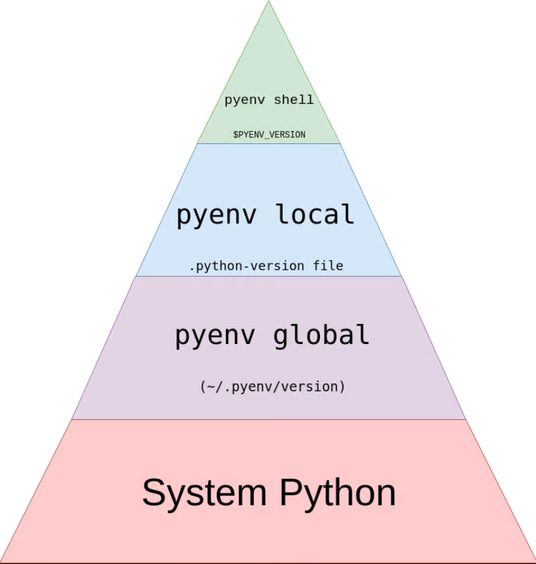
\includegraphics[width=0.5\textwidth]{IMG/pyenv.png} 
    \caption{Ordre de résolution des commandes \textbf{pyenv}}
\end{figure}

Voyons un exemple rapide :
\begin{lstlisting}[style=bash]
|\userprompt| pyenv versions
* system (set by /home/utilisateur/.pyenv/version)
  3.12.10
  3.14.0a7
\end{lstlisting}

Ici, c'est le système Python qui est utilisé.
\begin{lstlisting}[style=bash]
|\userprompt| pyenv global 3.14.0a7
|\userprompt| pyenv versions
  system
  3.12.10
* 3.14.0a7 (set by /home/utilisateur/.pyenv/version)
\end{lstlisting}

\textbf{pyenv} utilise maintenant \textbf{3.14.0a7} comme version de \textbf{Python}. Il indique même l'emplacement du fichier qu'il a trouvé. Ce fichier existe effectivement :
\begin{lstlisting}[style=bash]
|\userprompt| cat ~/.pyenv/version
3.14.0a7
\end{lstlisting}

Maintenant, créons un fichier \textbf{.python-version} avec \texttt{local} :
\begin{lstlisting}[style=bash]
|\userprompt| pyenv local 3.12.10
|\userprompt| pyenv versions
  system
* 3.12.10 (set by /home/utilisateur/.python-version)
  3.14.0a7
|\userprompt| cat .python-version
3.12.10
\end{lstlisting}

\textbf{pyenv} indique comment il doit résoudre la commande python. Cette fois, elle provient de \textbf{~/.python-version}. A Noter que la recherche de \textbf{.python-version} est récursive.
\begin{lstlisting}[style=bash]
|\userprompt| pyenv shell 3.14.0a7
|\userprompt| pyenv versions
  system
  3.12.10
* 3.14.0a7 (set by PYENV_VERSION environment variable)
\end{lstlisting}

Tout ce que cela a fait, c'est définir la variable d'environnement \texttt{\$PYENV\_VERSION} :
\begin{lstlisting}[style=bash]
|\userprompt| echo $PYENV_VERSION
3.14.0a7
\end{lstlisting}

\section{Environnement virtuel et \textit{pyenv}}
\textbf{pyenv} allié à un environnement virtuel est un mariage parfait. \textbf{pyenv} dispose d'un \textit{plugin} appelé \textbf{pyenv-virtualenv} qui permet de travailler avec plusieurs versions de Python et plusieurs environnements virtuels en un clin d'œil.
\begin{description}
    \item[pyenv] gère plusieurs versions de Python.
    \item[virtualenv/venv] gère les environnements virtuels pour une version spécifique de Python.
    \item[pyenv-virtualenv] gère les environnements virtuels pour différentes versions de Python.
\end{description}

\subsection*{Création d'un environnement virtuel}
\begin{lstlisting}[style=bash]
|\userprompt| pyenv virtualenv <version_python> <nom_environnement>
\end{lstlisting}

Une bonne pratique consiste à nommer les environnements du même nom que le projet. Par exemple, en travaillant sur \texttt{mon\_projet} développé avec \textbf{Python 3.6.8} :
\begin{lstlisting}[style=bash]
|\userprompt| pyenv virtualenv 3.6.8 mon_projet
\end{lstlisting}

\subsection*{Activation}
\begin{lstlisting}[style=bash]
|\userprompt| pyenv local mon_projet
\end{lstlisting}

Cela crée un fichier \textbf{.python-version} dans le répertoire de travail actuel et l'environnement sera automatiquement activé.

Vérification :
\begin{lstlisting}[style=bash]
|\userprompt| pyenv which python
/home/utilisateur/.pyenv/versions/my_project/bin/python
\end{lstlisting}

Une nouvelle version a été créée sous le nom de \texttt{my\_project} et l'exécutable python pointe vers cette version. En regardant n'importe quel exécutable fourni par cet environnement, nous verrons la même chose. Prenons, par exemple, \textbf{pip} :
\begin{lstlisting}[style=bash]
|\userprompt| pyenv which pip
/home/utilisateur/.pyenv/versions/my_project/bin/pip
\end{lstlisting}

Activer / Désactiver :
\begin{lstlisting}[style=bash]
|\userprompt| pyenv activate <nom_environnement>
|\userprompt| pyenv deactivate
\end{lstlisting}

\section{Travailler avec plusieurs environnements}
Supposons ces diverses versions de Python installées :
\begin{lstlisting}[style=bash]
|\userprompt| pyenv versions
* system (set by /home/user/.pyenv/version)
  3.11.12
  3.14.0a7
\end{lstlisting}

Par défaut, c'est le système Python qui est utilisé.

Nous souhaitons maintenant travailler sur deux projets différents :
\begin{itemize}
    \item \textbf{projet\_1}, qui supporte \textbf{Python 3.11.12}.
    \item \textbf{projet\_2}, qui supporte \textbf{Python 3.14.0a7}.
\end{itemize}

Créons un environnement virtuel pour chaque projet :
\begin{lstlisting}[style=bash]
|\userprompt| mkdir projet_1 projet_2
|\userprompt| cd projet_1
|\userprompt| pyenv which python3
/usr/bin/python3
|\userprompt| pyenv virtualenv 3.11.12 projet_01
|\userprompt| pyenv local projet_01
|\userprompt| python3 -V
Python 3.11.12
|\userprompt| cd ../projet_2
|\userprompt| pyenv which python3  # En changeant de répertoire on revient au système Python
/usr/bin/python3
|\userprompt| pyenv virtualenv 3.14.0a7 projet_02
|\userprompt| pyenv local projet_02
|\userprompt| python3 -V
Python 3.14.0a7
\end{lstlisting}

Plus besoin de se rappeler d'activer les environnements : en passant d'un projet à l'autre, \textbf{pyenv} se charge d'activer automatiquement les bonnes versions de Python et les bons environnements virtuels
\bigskip

\begin{center}
    \pgfornament[width=0.3\textwidth]{88} % 88 est le numéro de l'ornement
\end{center}

Nous venons d'explorer les multiples facettes de \textbf{pyenv}, un outil puissant qui permet de gérer efficacement différentes versions de Python. Grâce à \textbf{pyenv}, nous pouvons désormais basculer entre les versions de Python avec une facilité déconcertante, optimisant ainsi nos environnements de développement pour répondre aux besoins spécifiques de chaque projet. Cependant, la gestion des dépendances et des paquets reste un aspect crucial du développement Python. C'est là que \textbf{poetry} entre en jeu. Dans le chapitre suivant, nous plongerons dans les potentialités de \textbf{poetry}, un outil moderne qui simplifie la gestion des dépendances et des environnements virtuels, nous permettant de gérer nos projets Python avec une précision et une efficacité inégalées.


\chapter[\textit{poetry}]{\textit{poetry} \\ Un allié précieux \\ pour le développement Python}

\insertcitation{La poésie est ce qu'il y a de plus réel, c'est ce qui n'est complètement vrai que dans un autre monde.}{Charles Baudelaire}
\bigskip

\chapter[\textit{uv}]{\textit{uv} \\ Pour une gestion avancée \\ des environnements \\ de développement}

\insertcitation{Il y a un moyen de faire mieux, trouvez-le.}{Thomas Edison}
\bigskip

\textbf{uv} est un gestionnaire de dépendances ainsi qu'un outil de \textit{packaging} conçu pour offrir une performance optimale, tout en se révélant être d'une grande simplicité au niveau de son utilisation. \textbf{uv} se distingue par sa capacité à résoudre rapidement (écrit en \textbf{Rust}\footnote{\url{https://www.rust-lang.org/fr}} une attention fut portée sur la rapidité d'exécution) les dépendances et à créer des environnements virtuels de manière transparente.

Dans ce chapitre, nous allons explorer les grandes lignes de l'outil \textbf{uv} et découvrir comment il peut transformer notre approche du développement Python. Nous commencerons par une introduction à ses fonctionnalités de base, puis nous plongerons dans des aspects plus avancés, tels que la gestion des environnements virtuels, la résolution des dépendances, et le \textit{packaging} de projets, optimisant ainsi notre flux de travail.

Cet outil saura certainement devenir un allié incontournable, voire indispensable, pour notre boîte à outils de développement Python.

\section{Présentation d'\textit{uv}}
L'idée principale d'\textbf{uv} est d'accélérer le flux en accélérant les actions de gestion de projet. Par exemple, pour l'installation de paquets, \textbf{uv} est dix à cent fois plus rapide que \textbf{pip}.

\begin{figure}[h!]
    \centering
    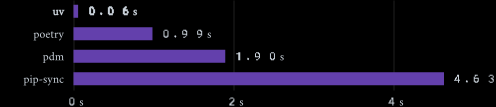
\includegraphics[width=0.7\textwidth]{IMG/uv_graph.png} % Remplacez par le chemin de votre image
    \caption{Graphique illustrant la rapidité, tiré de la documentation officielle}
\end{figure}

En outre, \textbf{uv} intègre dans un seul outil la plupart des fonctionnalités fournies par des outils tels que \textbf{pip}, \textbf{pip-tools}, \textbf{pipx}, \textbf{poetry}, \textbf{pyenv}, \textbf{twine}\footnote{\url{https://twine.readthedocs.io/en/stable/index.html}}, \textbf{virtualenv}, et bien d'autres encore. \textbf{uv} est donc une solution tout-en-un.

Caractéristiques d'\textbf{uv} :
\begin{itemize}
    \item Installation rapide des dépendances
    \item Gestion des environnements virtuels
    \item Gestion des versions de Python
    \item Initialisation du projet : Permet d'échafauder un projet Python complet, y compris le répertoire racine, le dépôt \textbf{Git}, l'environnement virtuel, \texttt{pyproject.toml}, \texttt{README}, etc.
    \item Gestion des dépendances pour une reproductibilité de l'environnement
    \item Gestion de la construction et de la publication des paquets
    \item Prise en charge des outils de développement : Installe et permet d'exécuter des outils de développement, tels que \textbf{pytest}\footnote{\url{https://docs.pytest.org/en/stable/}}, \textbf{Black}\footnote{\url{https://pypi.org/project/black/}} et \textbf{Ruff}\footnote{\url{https://docs.astral.sh/ruff/}}.
\end{itemize}
\medskip

Site officiel : \url{https://docs.astral.sh/uv/}

Serveur \textbf{Discord} : \url{https://discord.gg/JSsj35HH}

\section{Installation}
La façon la plus rapide (bien plus rapide) d'installer \textbf{uv} est d'utiliser l'installateur autonome fournit par le projet \textbf{uv}. Une autre option est d'installer \textbf{uv} à partir de \textbf{PyPI} en utilisant d'autres outils comme \textbf{pipx} ou \textbf{pip}\footnote{Pour d'autres modes d'installation voir la documentation officielle : \url{https://docs.astral.sh/uv/getting-started/installation/}}.

Pour installer la dernière version d'\textbf{uv} (sous forme de binaires) :
\begin{lstlisting}[style=bash]
|\userprompt| curl -LsSf https://astral.sh/uv/install.sh |\textbar| sh
downloading uv 0.7.8 x86_64-unknown-linux-gnu
no checksums to verify
installing to /home/user/.local/bin
  uv
  uvx
everything's installed!
\end{lstlisting}

Il est cependant possible d'obtenir une version spécifique d'\textbf{uv}\footnote{Voir la page \textbf{GitHub} des différentes versions : \url{https://github.com/astral-sh/uv/releases}} en incluant le numéro de version dans l'\textit{URL} :
\begin{lstlisting}[style=bash]
|\userprompt| curl -LsSf https://astral.sh/uv/0.7.7/install.sh |\textbar| sh
downloading uv 0.7.7 x86_64-unknown-linux-gnu
no checksums to verify
installing to /home/krystof/.local/bin
  uv
  uvx
everything's installed!
\end{lstlisting}

Vérifier l'installation :
\begin{lstlisting}[style=bash]
|\userprompt| uv --version 
uv 0.7.7
\end{lstlisting}

Activer l'auto-complétion dans \textbf{zsh}, à la fois pour \textbf{uv} et \textbf{uvx} :
\begin{lstlisting}[style=bash]
|\userprompt| echo 'eval "$(uv generate-shell-completion zsh)"' >> ~ /.zshrc
|\userprompt| echo 'eval "$(uvx generate-shell-completion zsh)"' >> ~/.zshrc
\end{lstlisting}

\subsection*{Mise à jour d'\textit{uv}}
Comme le projet \texttt{uv} est en développement actif, de nouvelles versions sont régulièrement publiées. Si \textbf{uv} a été installé à l'aide de l'installateur autonome il sera nécessaire d'exécuter la commande suivante :
\begin{lstlisting}[style=bash]
|\userprompt| uv self update
info: Checking for updates...
success: Upgraded uv from v0.7.7 to v0.7.8! https://github.com/astral-sh/uv/releases/tag/0.7.8
\end{lstlisting}

\subsection*{Désinstallation}
Nettoyer les données stockées :
\begin{lstlisting}[style=bash]
|\userprompt| uv cache clean
No cache found at: .cache/uv  # Normal au début
|\userprompt| rm -r "$(uv python dir)"
|\userprompt| rm -r "$(uv tool dir)"
\end{lstlisting}

Supprimer les binaires \textbf{uv} et \textbf{uvx} :
\begin{lstlisting}[style=bash]
|\userprompt| rm ~/.local/bin/uv ~/.local/bin/uvx
|\userprompt| uv --version
zsh: command not found: uv
\end{lstlisting}

\subsection*{Un aperçu rapide}
Maintenant qu'\textbf{uv} est installé prenons le temps de visualiser très rapidement ce que cet outil a à nous proposer :
\begin{lstlisting}[style=bash]
|\userprompt| uv
An extremely fast Python package manager.

Usage: uv [OPTIONS] <COMMAND>

Commands:
  run      Run a command or script
  init     Create a new pyproject
# Saisir la commande pour voir la suite de la sortie...
\end{lstlisting}

Pour accéder à l'aide d'une commande d'\textbf{uv} :
\begin{lstlisting}[style=bash]
|\userprompt| uv --help <commande>
\end{lstlisting}

Par exemple, la commande \texttt{cache} :
\begin{lstlisting}[style=bash]
|\userprompt| uv --help cache
\end{lstlisting}

Cela permet d'ouvrir un visualisateur dans lequel on retrouve les informations sollicitées (ce qui suit n'est qu'un extrait) :
\begin{lstlisting}[style=visual]
Manage uv's cache

Usage: uv cache [OPTIONS] <COMMAND>

Commands:
  clean  Clear the cache, removing all entries or those linked to specific packages
  prune  Prune all unreachable objects from the cache
  dir    Show the cache directory
|\textcolor{nord4}{[...]}|
\end{lstlisting}

\section{La gestion de projet}

Pour cette section et la suite du didacticiel, nous utiliserons un exemple d'application qui permet d'afficher un calendrier à l'aide d'une interface graphique créée via le \textit{framework} \textbf{Qt for Python}\footnote{\url{https://doc.qt.io/qtforpython-6/}, alias \textbf{PySide6} : \url{https://pypi.org/project/PySide6/}}. Le code de cette application se trouve sur un dépôt \textbf{GitHub}\footnote{\url{https://github.com/Krystof2so/PyCalendar} - Voir également l'annexe \textit{Code du projet \textbf{Calendar}} page \pageref{code_calendar}}. Il s'agit d'un petit projet personnel réalisé au cours de mon apprentissage du \textit{framework}, mais rien ne vous empêche de tester toutes les manipulations qui vont suivre à partir de tout autre projet. Le projet \textbf{Calendar} ne me sert qu'à illustrer mon propos.

Créer et travailler sur des projets Python avec \textbf{uv}, revient à travailler avec le fichier \texttt{pyproject.toml}, fichier qui, comme nous l'avons vu dans les chapitres précédents, définit les dépendances.

\subsection*{Création d'un projet}

Pour créer et initialiser un projet Python avec \textbf{uv}, naviguer jusqu'au répertoire dans lequel on souhaite stocker le projet (par exemple le répertoire personnel de l'utilisateur), puis exécuter la commande :
\begin{lstlisting}[style=bash]
|\userprompt| uv init mon_projet
Initialized project `mon_projet` at `/home/utilisateur/mon_projet`
\end{lstlisting}

ou bien :
\begin{lstlisting}[style=bash]
|\userprompt| mkdir mon_projet
|\userprompt| cd mon_projet
|\userprompt| uv init
Initialized project `mon_projet`
\end{lstlisting}

Cela crée dans le répertoire du projet (\texttt{mon\_projet}) la structure suivante :
\begin{lstlisting}[style=tree]
mon_projet/
|\textbar|
|\textbar|--.python-version
|\textbar|--README.md
|\textbar|--main.py
|\textbar|--pyproject.toml
\end{lstlisting}

Le fichier \texttt{.python-version} contient la version de Python par défaut pour le projet en cours. Ce fichier indique à \textbf{uv} la version de Python à utiliser lors de la création d'un environnement virtuel dédié au projet. Ensuite, il y a un fichier \texttt{README.md}.  Et l'on trouve un fichier \texttt{main.py} qui contient les lignes suivantes :
\begin{lstlisting}[style=python]
def main():
    print("Hello from mon-projet!")


if __name__ == "__main__":
    main()
\end{lstlisting}

Et au final un fichier \texttt{pyproject.toml} initié avec une configuration basique :
\begin{lstlisting}[style=file]
[project]
name = "mon-projet"
version = "0.1.0"
description = "Add your description here"
readme = "README.md"
requires-python = ">=3.13"
dependencies = []
\end{lstlisting}

Nous pouvons changer la description :
\begin{lstlisting}[style=file]
description = "Un simple projet"
\end{lstlisting}


\subsection*{Initier un projet existant}
Nous allons pour cela utiliser le projet \textbf{Calendar}\footnote{Cf. annexe \textit{Code du projet \textbf{Calendar}} page \pageref{code_calendar}}. Il suffit tout simplement de se rendre dans le répertoire du projet et de lancer la commande \texttt{init} :
\begin{lstlisting}[style=bash]
|\userprompt| uv init
Initialized project `calendar`
|\userprompt| tree  
.
|\textbar|-- IMG
|\textbar|   |\textbar|-- PyCalendar.png
|\textbar|-- main.py
|\textbar|-- pyproject.toml
|\textbar|-- README.md
|\textbar|-- src
|\textbar|-- pycalendar
        |\textbar|-- main.py

4 directories, 5 files
\end{lstlisting}

Cette commande va seulement générer le fichier \texttt{pyproject.toml}. Elle ne va ni écraser, ni modifier les fichiers existants, ni modifier la structure du projet. Cependant, cette commande ne fonctionnera pas si un fichier \texttt{pyproject.toml} est déjà présent. Si c'est le cas, copier le fichier avant de lancer la commande \texttt{uv init}, il pourra servir pour modifier le nouveau fichier généré avec toute configuration pertinente de l'ancien \texttt{pyproject.toml}.

\subsection*{Exécution du script d'entrée du projet}
\begin{lstlisting}[style=bash, escapeinside={||}]
|\userprompt| uv run main.py
Using CPython 3.13.3 interpreter at: /usr/bin/python3.13
Creating virtual environment at: .venv
Hello from calendar!
|\userprompt| tree -a
.
|\textbar|-- main.py
|\textbar|-- pyproject.toml
|\textbar|-- .python-version
|\textbar|-- README.md
|\textbar|-- uv.lock
|\textbar|-- .venv
    |\textbar|-- bin
    |\textbar|   |\textbar|-- activate
    |\textbar|   |\textbar|-- activate.bat
    |\textbar|   |\textbar|-- activate.csh
    |\textbar|   |\textbar|-- activate.fish
    |\textbar|   |\textbar|-- activate.nu
    |\textbar|   |\textbar|-- activate.ps1
    |\textbar|   |\textbar|-- activate_this.py
    |\textbar|   |\textbar|-- deactivate.bat
    |\textbar|   |\textbar|-- pydoc.bat
    |\textbar|   |\textbar|-- python -> /usr/bin/python3.13
    |\textbar|   |\textbar|-- python3 -> python
    |\textbar|   |\textbar|-- python3.13 -> python
    |\textbar|-- CACHEDIR.TAG
    |\textbar|-- .gitignore
    |\textbar|-- lib
    |\textbar|   |\textbar|-- python3.13
    |\textbar|       |\textbar|-- site-packages
    |\textbar|           |\textbar|-- __pycache__
    |\textbar|           |\textbar|   |\textbar|-- _virtualenv.cpython-313.pyc
    |\textbar|           |\textbar|-- _virtualenv.pth
    |\textbar|           |\textbar|-- _virtualenv.py
    |\textbar|-- lib64 -> lib
    |\textbar|-- pyvenv.cfg

8 directories, 23 files
\end{lstlisting}

La première fois que l'on exécutez une commande de projet, soit \texttt{uv run}, \texttt{uv sync} (création de l'environnement du projet) ou \texttt{uv lock}, la version de Python utilisée pour le projet est affichée. \textbf{uv} crée ensuite un environnement virtuel et un fichier \texttt{uv.lock} (cf. infra) à la racine du projet, ainsi qu'un fichier \texttt{.gitignore}, installé dans le répertoire de gestion de l'environnement virtuel (\texttt{.venv}) dont le contenu est vide. 

Si l'on ne souhaite pas qu'\textbf{uv} gère l'environnement du projet, désactiver le verrouillage et la synchronisation automatiques du projet dans \texttt{pyproject.toml} :
\begin{lstlisting}[style=file]
[tool.uv]
managed = false
\end{lstlisting}

Ce qui donnera à la première exécution :
\begin{lstlisting}[style=bash]
|\userprompt| uv run main.py
Hello from mon_projet!
|\userprompt| tree -a
.
|\textbar|-- main.py
|\textbar|-- pyproject.toml
|\textbar|-- .python-version
|\textbar|-- README.md

1 directory, 4 files
\end{lstlisting}

\section{La gestion des dépendances}
\subsection*{Ajout et installation des dépendances}
Revenons au projet \textbf{Calendar} :
\begin{lstlisting}[style=bash]
|\userprompt| cd calendar
|\userprompt| uv init
Initialized project `calendar`
|\userprompt| uv run src/pycalendar/main.py
Using CPython 3.13.3 interpreter at: /usr/bin/python3.13
Creating virtual environment at: .venv
Traceback (most recent call last):
  File "/home/utilisateur/calendar/src/pycalendar/main.py", line 4, in <module>
    from PySide6.QtCore import QSize, Qt
ModuleNotFoundError: No module named 'PySide6'
\end{lstlisting}

L'exception levée est sans appel : il nous manque un module nécessaire pour exécuter correctement notre application, le module \textbf{PySide6}. Remédions à cela:
\begin{lstlisting}[style=bash]
|\userprompt| uv add pyside6
Resolved 5 packages in 443ms
Prepared 4 packages in 10.63s
Installed 4 packages in 146ms
 + pyside6==6.9.0
 + pyside6-addons==6.9.0
 + pyside6-essentials==6.9.0
 + shiboken6==6.9.0
\end{lstlisting}

Ou bien en spécifiant une version précise du module :
\begin{lstlisting}[style=bash]
|\userprompt| uv add "pyside6==6.9.0"
Resolved 10 packages in 16ms
Installed 4 packages in 117ms
 + pyside6==6.9.0
 + pyside6-addons==6.9.0
 + pyside6-essentials==6.9.0
 + shiboken6==6.9.0
\end{lstlisting}

Ces commandes permettent d'ajouter la bibliothèque \textbf{PySide6} aux dépendances du projet et de l'installer dans l'environnement virtuel. Le fichier \texttt{pyproject.toml} est alors modifié en conséquence :
\begin{lstlisting}[style=file]
[project]
name = "calendar"
version = "0.1.0"
description = "Simple calendar"
readme = "README.md"
requires-python = ">=3.13"
dependencies = [
    "pyside6>=6.9.0",
]
\end{lstlisting}

Il est même possible d'ajouter une dépendance depuis un projet \textbf{GitHub} (par exemple , le module \textbf{requests}) :
\begin{lstlisting}[style=bash]
|\userprompt| uv add git+https://github.com/psf/requests
    Updated https://github.com/psf/requests (c65c780849563c891f35ffc98d3198b71011c012)
Resolved 15 packages in 364ms
      Built requests @ git+https://github.com/psf/requests@c65c780849563c891f35ffc98d3198b71011c 012
Prepared 5 packages in 891ms
Installed 5 packages in 7ms
 + certifi==2025.4.26
 + charset-normalizer==3.4.2
 + idna==3.10
 + requests==2.32.3 (from git+https://github.com/psf/requests@c65c780849563c891f35ffc98d3198b71011c012)
 + urllib3==2.4.0
\end{lstlisting}

Si le projet possédait déjà un fichier \texttt{requirements.txt} : 
\begin{lstlisting}[style=file]
PySide6==6.9.0
PySide6_Addons==6.9.0
PySide6_Essentials==6.9.0
shiboken6==6.9.0
\end{lstlisting}

Il suffisait alors d'en passer par lui :
\begin{lstlisting}[style=bash]
|\userprompt| uv add -r requirements.txt
Using CPython 3.13.3 interpreter at: /usr/bin/python3.13
Creating virtual environment at: .venv
Resolved 5 packages in 1ms
Installed 4 packages in 91ms
 + pyside6==6.9.0
 + pyside6-addons==6.9.0
 + pyside6-essentials==6.9.0
 + shiboken6==6.9.0
\end{lstlisting}

Et notre nouveau \texttt{pyproject.toml}:
\begin{lstlisting}[style=file]
[project]
name = "calendar"
version = "0.1.0"
description = "Add your description here"
readme = "README.md"
requires-python = ">=3.13"
dependencies = [
    "pyside6==6.9.0",
    "pyside6-addons==6.9.0",
    "pyside6-essentials==6.9.0",
    "shiboken6==6.9.0",
]
\end{lstlisting}

\textit{uv add} met également à jour le fichier \texttt{uv.lock} avec les informations de version pour les éléments suivants :
\begin{description}
    \item[Dépendances directes] : paquets dont le projet dépend directement (\textbf{pyside6}). 
    \item[Dépendances transitives] : paquets qui prennent en charge les dépendances directes du projet (les trois autres).
\end{description}

\texttt{uv add} fait intégralement le travail de gestion des dépendances en les installant, en éditant le fichier \texttt{pyproject.toml} et en maintenant le fichier \texttt{uv.lock} à jour. Cela garantit une reproductibilité de l'environnement de travail.

Une fois les dépendances installées, nous pouvons relancer notre script.

\subsection*{Mise à jour et suppression des dépendances}
Mise à jour d'un paquet :
\begin{lstlisting}[style=bash]
|\userprompt| uv add --upgrade pyside6  # Ici nous avons déjà la dernière version
Resolved 5 packages in 158ms
Audited 4 packages in 0.97ms
\end{lstlisting}

Ou bien :
\begin{lstlisting}[style=bash]
|\userprompt|uv lock --upgrade-package pyside6
Resolved 15 packages in 756ms
\end{lstlisting}

Suppression d'une dépendance :
\begin{lstlisting}[style=bash]
|\userprompt| uv remove pyside6
Resolved 1 package in 11ms
Uninstalled 4 packages in 66ms
 - pyside6==6.9.0
 - pyside6-addons==6.9.0
 - pyside6-essentials==6.9.0
 - shiboken6==6.9.0
\end{lstlisting}

Il est important de noter que \texttt{uv remove} supprime également les dépendances transitives et met à jour les fichiers \texttt{pyproject.toml} et \texttt{uv.lock} en conséquence.

\subsection*{Les dépendances de développement}
Les bibliothèques de test comme \textbf{pytest}, les formateurs de code comme \textbf{Ruff} et les vérificateurs de types statiques comme \textbf{mypy} font partie de ces dépendances de développement. On les installe à l'aide de la commande \texttt{uv add --dev paquet} :
\begin{lstlisting}[style=bash]
|\userprompt| uv add --dev pytest
Resolved 10 packages in 335ms
Prepared 4 packages in 137ms
Installed 4 packages in 21ms
 + iniconfig==2.1.0
 + packaging==25.0
 + pluggy==1.5.0
 + pytest==8.3.5
\end{lstlisting}

Cette commande installe \textbf{pytest} dans l'environnement virtuel du projet et ajoute la bibliothèque comme dépendance de développement aux fichiers \texttt{pyproject.toml} et \texttt{uv.lock}. Lignes ajoutées dans \texttt{pyproject.toml}:
\begin{lstlisting}[style=file]
[dependency-groups]
dev = [
    "pytest>=8.3.5",
]
\end{lstlisting}

\subsection*{Verrouillage et synchronisation de l'environnement}
Le verrouillage consiste à capturer les dépendances spécifiques du projet dans le fichier \texttt{uv.lock} qui est un fichier de verrouillage multi-plateforme contenant des informations précises sur les dépendances du projet, c'est-à-dire les versions exactes résolues qui sont installées dans l'environnement du projet. Ce fichier doit être vérifié dans le contrôle de version, ce qui permet des installations cohérentes et reproductibles sur toutes les machines. Ce processus permet donc de reproduire un environnement de travail dans toutes les configurations possibles, y compris la version et la distribution de Python, le système d'exploitation et l'architecture. Ce fichier est directement géré par \textbf{uv}. Par exemple, lorsque l'on exécute \texttt{uv run}, le projet est verrouillé et synchronisé avant que la commande ne soit invoquée. Ce comportement garantit que l'environnement du projet reste toujours à jour. Il sera nécessaire d'enregistrer ce fichier dans le système de contrôle de version. Un tel fichier ne doit pas être édité manuellement.

Nous pouvez explicitement verrouiller et synchroniser notre projet avec les commandes suivantes :
\begin{lstlisting}[style=bash]
|\userprompt| uv lock
Resolved 5 packages in 0.93ms
$ uv sync
Resolved 5 packages in 1ms
Audited 4 packages in 0.01ms
\end{lstlisting}

Ces commandes sont utiles si nous rencontrons des problèmes lors de l'exécution du projet et pour s'assurer que nous utilisons la bonne version de chaque dépendance.

Imaginons un projet cloné depuis un dépôt distant (comme \textbf{GitHub}), qui ne contient donc pas le répertoire de l'environnement virtuel. Il nous suffit de lancer depuis le répertoire racine du projet :
\begin{lstlisting}[style=bash]
|\userprompt| uv run src/pycalendar/main.py
Using CPython 3.13.3 interpreter at: /usr/bin/python3.13
Creating virtual environment at: .venv
Installed 13 packages in 96ms
\end{lstlisting}

Avant d'essayer d'exécuter l'application, \textbf{uv} crée un environnement virtuel dans le répertoire \texttt{.venv/}. Il installe ensuite les dépendances et exécute enfin l'application.

Pour vérifier quels modules sont présents au niveau de notre environnement virtuel :
\begin{lstlisting}[style=bash]
|\userprompt| uv pip list
Package            Version
------------------ -------
pyside6            6.9.0
pyside6-addons     6.9.0
pyside6-essentials 6.9.0
shiboken6          6.9.0
\end{lstlisting}

Nous pouvons comparer cette liste avec le contenu du fichier \texttt{uv.lock}.

Note : une visualisation sous la forme d'une arborescence (tout en mettant le fichier de verrouillage à jour):
\begin{lstlisting}[style=bash]
|\userprompt| uv tree
Resolved 5 packages in 1ms
calendar v0.1.0
|\textbar|-- pyside6 v6.9.0
    |\textbar|-- pyside6-addons v6.9.0
    |\textbar|   |\textbar|-- pyside6-essentials v6.9.0
    |\textbar|   |\textbar|     |\textbar|-- shiboken6 v6.9.0
    |\textbar|   |\textbar|-- shiboken6 v6.9.0
    |\textbar|-- pyside6-essentials v6.9.0 (*)
    |\textbar|-- shiboken6 v6.9.0
(*) Package tree already displayed
\end{lstlisting}

\subsubsection*{Les options de désactivation et de non-vérification}
Pour désactiver le verrouillage automatique, utiliser l'option \texttt{--locked} :
\begin{lstlisting}[style=bash]
|\userprompt| uv run src/pycalendar/main.py --locked
|\userprompt|
\end{lstlisting}

Si le fichier de verrouillage n'est pas à jour, \textbf{uv} lèvera une erreur au lieu de mettre à jour le fichier de verrouillage.

Utiliser le fichier de verrouillage sans vérifier s'il est à jour :
\begin{lstlisting}[style=bash]
|\userprompt| uv run src/pycalendar/main.py --frozen
|\userprompt|
\end{lstlisting}

De même, pour exécuter une commande sans vérifier si l'environnement est à jour :
\begin{lstlisting}[style=bash]
|\userprompt| uv run --no-sync src/pycalendar/main.py
|\userprompt|
\end{lstlisting}

\subsubsection*{Le fichier \textit{pylock.toml}}
A ce sujet on se réfèrerar au \textbf{PEP 751}\footnote{Un format de fichier pour enregistrer les dépendances de Python pour la reproductibilité de l'installation : \url{https://peps.python.org/pep-0751/}}.

\texttt{pylock.toml} est un format de sortie de résolution destiné à remplacer \texttt{requirements\\.txt}. \texttt{pylock.toml} est standardisé et agnostique, de sorte qu'à l'avenir, les fichiers \texttt{pylock\\.toml} générés par \textbf{uv} pourraient être installés par d'autres outils, et vice-versa. Mais ce format demeure encore expérimental et n'est pas pleinement opérationnel.

Pour exporter un \texttt{uv.lock} au format \texttt{pylock.toml} (nécessite l'existence du fichier \texttt{pyp\\roject.toml}) : 
\begin{lstlisting}[style=bash]
|\userprompt| uv export -o pylock.toml
Resolved 5 packages in 2ms
# This file was autogenerated by uv via the following command:
#    uv export -o pylock.toml
lock-version = "1.0"
created-by = "uv"
requires-python = ">=3.13"

[[packages]]
name = "pyside6"
version = "6.9.0"
index = "https://pypi.org/simple"
[...]
\end{lstlisting}

\section{Les commandes}
\begin{table}[h!]
\centering
\begin{tabular}{|l|p{12cm}|}
\hline
\textbf{Commandes} & \textbf{Description} \\
\hline
\texttt{uv init} & Créer un nouveau projet Python. \\
\hline
\texttt{uv add} & Ajouter une dépendance au projet. \\
\hline
\texttt{uv remove} & Supprime une dépendance du projet. \\
\hline
\texttt{uv sync} & Synchronise les dépendances du projet avec l'environnement. \\
\hline
\texttt{uv lock} & Créer un fichier de verrouillage pour les dépendances du projet. \\
\hline
\texttt{uv run} & Exécuter une commande dans l'environnement du projet. \\
\hline
\texttt{uv tree} & Affiche l'arbre des dépendances du projet. \\
\hline
\texttt{uv build} & Construire le projet dans des archives de distribution. \\
\hline
\texttt{uv publish} & Publier le projet dans un index de paquets. \\
\hline
\end{tabular}
    \caption{Commandes et leur description pour créer un projet Python avec \textbf{uv}}
\end{table}
\bigskip

\begin{center}
    \pgfornament[width=0.3\textwidth]{88} % 88 est le numéro de l'ornement
\end{center}

Nous venons d'explorer en détail les multiples facettes de l'outil \textbf{uv}, un outil innovant qui transforme notre approche de la gestion des dépendances et des environnements de développement Python. Que l'on travaille sur des projets de petite ou de grande envergure, \textbf{uv} s'adapte à nos besoins et nous permet de nous concentrer sur l'essentiel : le développement. 

En intégrant \textbf{uv} à notre boîte à outils de développement, nous optimisons notre flux de travail. Les fonctionnalités avancées de \textbf{uv}, telles que la résolution rapide des dépendances et la gestion simplifiée des environnements virtuels, en font un allié incontournable pour tout développeur Python soucieux d'efficacité et de qualité.



% Annexes :
\backmatter
\addcontentsline{toc}{part}{Annexes}
\part*{\textcolor{nord11}{Annexes}}
\chapter{Code du projet \textit{Calendar}}\label{code_calendar}

Voici le code Python du projet \textbf{Calendar}\footnote{Egalement disponible sur \textbf{Github} : \url{https://github.com/Krystof2so/PyCalendar}. Il se peut que sur le dépôt \textbf{Github} le code différe, le principe reste cependant le même, mais vous pouvez aussi utiliser l'exemple tel que fourni dans cette annexe} :

\begin{lstlisting}[style=python]
import calendar

from datetime import datetime
from PySide6.QtCore import QSize, Qt
from PySide6.QtWidgets import QApplication, QWidget, QVBoxLayout, QHBoxLayout,\
                              QGridLayout, QLabel, QPushButton
from PySide6.QtGui import QPalette, QColor


DAYS_OF_WEEK = ("Lundi", "Mardi", "Mercredi", "Jeudi", "Vendredi", "Samedi", "Dimanche")


class CalendarApp(QWidget):   
    def __init__(self):
        super().__init__()

        self.setWindowTitle("PyCalendar")
        self.setGeometry(100, 100, 400, 300)

         # Initialiser la date actuelle :
        self.current_date = datetime.now()

        # Layout vertical principal :
        main_layout = QVBoxLayout()
        self.setLayout(main_layout)

        # Layout horizontal pour afficher le mois en cours et les boutons de navigation:
        month_layout = QHBoxLayout()
        main_layout.addLayout(month_layout)

        # Bouton pour le mois précédent :
        self.prev_button = QPushButton("<")
        self.prev_button.setFixedSize(QSize(30, 30))  # Définir une taille fixe pour le bouton
        self.prev_button.clicked.connect(self.show_previous_month)
        month_layout.addWidget(self.prev_button)

        # QLabel pour afficher le mois en cours :
        self.month_label = QLabel(self.get_current_month_year())
        self.month_label.setAlignment(Qt.AlignCenter)
        month_layout.addWidget(self.month_label)

        # Bouton pour le mois suivant :
        self.next_button = QPushButton(">")
        self.next_button.setFixedSize(QSize(30, 30))  # Définir une taille fixe pour le bouton
        self.next_button.clicked.connect(self.show_next_month)
        month_layout.addWidget(self.next_button)

        # Ajouter la grille du calendrier :
        self.calendar_layout = QGridLayout()
        main_layout.addLayout(self.calendar_layout)

        # Remplir la grille avec les jours du mois :
        self.populate_calendar()

    def get_current_month_year(self):
        return self.current_date.strftime("%B %Y")

    def is_today(self, day):
        """Vérifie si le jour donné est aujourd'hui."""
        today = datetime.now()
        return day == today.day and self.current_date.month == today.month and self.current_date.year == today.year

    def populate_calendar(self):
        """Obtenir les jours du mois, et les placer dans la grille."""
        year = self.current_date.year
        month = self.current_date.month
        cal = calendar.monthcalendar(year, month)
        # Effacer la grille précédente :
        self.clear_layout(self.calendar_layout)
        # Ajouter les jours de la semaine :
        for col, day_label in enumerate(DAYS_OF_WEEK):
            label = QLabel(day_label[0:2])
            label.setAlignment(Qt.AlignCenter)
            self.calendar_layout.addWidget(label, 0, col)
        # Ajouter les jours du mois :
        for row, week in enumerate(cal):
            for col, day in enumerate(week):
                label = QLabel("" if day == 0 else str(day))
                label.setAlignment(Qt.AlignCenter)
                if self.is_today(day):
                    palette = label.palette()
                    palette.setColor(QPalette.WindowText, QColor('#A3BE8C'))  # Vert du thème Nord
                    label.setPalette(palette)
                self.calendar_layout.addWidget(label, row + 1, col)

    def clear_layout(self, layout):
        """Effacer tous les widgets d'un layout."""
        while layout.count():
            child = layout.takeAt(0)
            if child.widget():
                child.widget().deleteLater()

    def show_previous_month(self):
        """Afficher le mois précédent."""
        if self.current_date.month == 1:
            self.current_date = self.current_date.replace(year=self.current_date.year - 1, month=12)
        else:
            self.current_date = self.current_date.replace(month=self.current_date.month - 1)
        self.month_label.setText(self.get_current_month_year())
        self.populate_calendar()

    def show_next_month(self):
        """Afficher le mois suivant."""
        if self.current_date.month == 12:
            self.current_date = self.current_date.replace(year=self.current_date.year + 1, month=1)
        else:
            self.current_date = self.current_date.replace(month=self.current_date.month + 1)
        self.month_label.setText(self.get_current_month_year())
        self.populate_calendar()

if __name__ == "__main__":
    app = QApplication([])
    window = CalendarApp()
    window.show()
    app.exec()
\end{lstlisting}

Voici une image de ce que ce code propose :
\begin{figure}[h!]
    \centering
    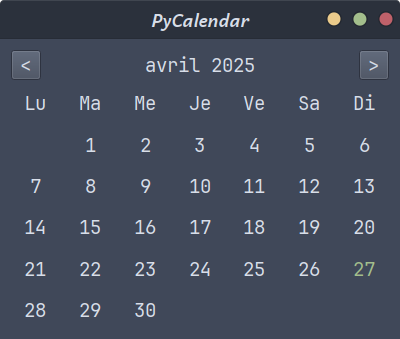
\includegraphics[width=0.6\textwidth]{IMG/PyCalendar.png}
    \caption{Application \textbf{Calendar}}
\end{figure}

L'arborescence du projet est la suivante :
\begin{lstlisting}[style=tree]
Calendar
|\textbar|-- IMG
|\textbar|   |\textbar|-- PyCalendar.png
|\textbar|-- README.md
|\textbar|-- src
    |\textbar|-- pycalendar
        |\textbar|-- main.py
\end{lstlisting}


\end{document}
